%%%%%%%%%%%%%%%%%%%%%%%%%%%%% Thesis.tex %%%%%%%%%%%%%%%%%%%%%%%%%%%%%%%
%                                                                      %
%  ---------- Master of Science Dissertation template ----------       %
%                                                                      %
%  Template for the Master Thesis according to the regulations         %
%  published by the Academic Board (Direcção Académica) at IST.        %
%                                                                      %
%  For up-to-date guide, please refer to the official website          %
%  http://academica.tecnico.ulisboa.pt/alunos/dissertacao-de-mestrado/ %
%                                                                      %
%       Andre C. Marta                                                 %
%       Area Cientifica de Mecanica Aplicada e Aeroespacial            %
%       Departamento de Engenharia Mecanica                            %
%       Instituto Superior Tecnico                                     %
%       Av. Rovisco Pais                                               %
%       1049-001 Lisboa                                                %
%       Portugal                                                       %
%       Tel: +351 21 841 9469                                          %
%                        3469 (extension)                              %
%       Email: andre.marta@tecnico.ulisboa.pt                          %
%                                                                      %
%  Created:       Jan 20, 2011                                         %
%  Last Modified: Feb 19, 2018                                         %
%                                                                      %
%%%%%%%%%%%%%%%%%%%%%%%%%%%%%%%%%%%%%%%%%%%%%%%%%%%%%%%%%%%%%%%%%%%%%%%%
%  Revision history                                                    %
%  v1 - 2011/01/24 - original template                                 %
%  v2 - 2012/10/30 - new IST image and glossary support                %
%  v3 - 2013/12/10 - update according to 2012/13 official guide        %
%  v4 - 2014/02/28 - new default for bibliography style                %
%  v5 - 2014/05/07 - update according to 2013/14 official guide        %
%  v6 - 2015/07/02 - cover page format fixed,                          %
%                    contents page numbering fixed,                    %
%                    better language support,                          %
%                    enhanced examples of tables,                      %
%                    new option for appendix page numbering format,    %
%                    custom bibliography style                         %
%  v7 - 2018/02/19 - multiple citations compressed                     %
%%%%%%%%%%%%%%%%%%%%%%%%%%%%%%%%%%%%%%%%%%%%%%%%%%%%%%%%%%%%%%%%%%%%%%%%
%                                                                      %
% To generate the PDF file, type "make" at the terminal prompt.        %
%                                                                      %
% The IST template LaTeX package was created by the author             %
% and it can be downloaded from:                                       %
% https://fenix.ist.utl.pt/homepage/ist31052/                          %
%                                                                      %
% The external packages can be downloaded from                         %
% the Comprehensive TeX Archive Network at http://www.ctan.org/        %
%                                                                      %
% List of LaTex symbols:                                               %
% http://www.ctan.org/tex-archive/info/symbols/comprehensive/          %
%                                                                      %
% Help with LaTex can be found at                                      %
% http://www.giss.nasa.gov/tools/latex/ltx-2.html                      %
% http://en.wikibooks.org/wiki/LaTeX                                   %
%%%%%%%%%%%%%%%%%%%%%%%%%%%%%%%%%%%%%%%%%%%%%%%%%%%%%%%%%%%%%%%%%%%%%%%%

%%%%%%%%%%%%%%%%%%%%%%%%%%%%%%%%%%%%%%%%%%%%%%%%%%%%%%%%%%%%%%%%%%%%%%%%
%     Preamble                                                         %
%%%%%%%%%%%%%%%%%%%%%%%%%%%%%%%%%%%%%%%%%%%%%%%%%%%%%%%%%%%%%%%%%%%%%%%%

% ----------------------------------------------------------------------
%  Set the document class
% ----------------------------------------------------------------------
\documentclass[10pt,a4paper,twoside]{report}

% ----------------------------------------------------------------------
% Define external packages, language, margins, fonts and new commands
% ----------------------------------------------------------------------
%%%%%%%%%%%%%%%%%%%%%%%%%%%%%%%%%%%%%%%%%%%%%%%%%%%%%%%%%%%%%%%%%%%%%%%%
%                                                                      %
%     File: Thesis_Preamble.tex                                        %
%     Tex Master: Thesis.tex                                           %
%                                                                      %
%     Author: Andre C. Marta                                           %
%     Last modified : 9 Apr 2015                                       %
%                                                                      %
%%%%%%%%%%%%%%%%%%%%%%%%%%%%%%%%%%%%%%%%%%%%%%%%%%%%%%%%%%%%%%%%%%%%%%%%

% ----------------------------------------------------------------------
% Define document language.
% ----------------------------------------------------------------------

% 'inputenc' package
%
% Accept different input encodings.
% http://www.ctan.org/tex-archive/macros/latex/base/
%
% > allows typing non-english text in LaTeX sources.
%
% ******************************* SELECT *******************************
%\usepackage[latin1]{inputenc} % <<<<< Windows
\usepackage[utf8]{inputenc}   % <<<<< Linux
% ******************************* SELECT *******************************


% 'babel' package
%
% Multilingual support for Plain TeX or LaTeX.
% http://www.ctan.org/tex-archive/macros/latex/required/babel/
%
% > sets the variable names according to the language selected
%
% ******************************* SELECT *******************************
%\usepackage[portuguese]{babel} % <<<<< Portuguese
\usepackage[english]{babel} % <<<<< English
% ******************************* SELECT *******************************


% List of LaTeX variable names: \abstractname, \appendixname, \bibname,
%   \chaptername, \contentsname, \listfigurename, \listtablename, ...)
% http://www.tex.ac.uk/cgi-bin/texfaq2html?label=fixnam
%
% Changing the words babel uses (uncomment and redefine as necessary...)
%
\newcommand{\acknowledgments}{@undefined} % new LaTeX variable name
%
% > English
%
\addto\captionsenglish{\renewcommand{\acknowledgments}{Acknowledgments}}
%\addto\captionsenglish{\renewcommand{\contentsname}{Contents}}
%\addto\captionsenglish{\renewcommand{\listtablename}{List of Tables}}
%\addto\captionsenglish{\renewcommand{\listfigurename}{List of Figures}}
%\addto\captionsenglish{\renewcommand{\nomname}{Nomenclature}}
%\addto\captionsenglish{\renewcommand{\glossaryname}{Glossary}}
%\addto\captionsenglish{\renewcommand{\acronymname}{List of Acronyms}}
%\addto\captionsenglish{\renewcommand{\bibname}{References}} % Bibliography
%\addto\captionsenglish{\renewcommand{\appendixname}{Appendix}}

% > Portuguese
%
\addto\captionsportuguese{\renewcommand{\acknowledgments}{Agradecimentos}}
%\addto\captionsportuguese{\renewcommand{\contentsname}{Conte\'{u}do}}
%\addto\captionsportuguese{\renewcommand{\listtablename}{Lista de Figuras}}
%\addto\captionsportuguese{\renewcommand{\listfigurename}{Lista de Tabelas}}
\addto\captionsportuguese{\renewcommand{\nomname}{Lista de S\'{i}mbolos}} % Nomenclatura
%\addto\captionsportuguese{\renewcommand{\glossary}{Gloss\'{a}rio}}
%\addto\captionsportuguese{\renewcommand{\acronymname}{Lista de Abrevia\c{c}\~{o}es}}
%\addto\captionsportuguese{\renewcommand{\bibname}{Refer\^{e}ncias}} % Bibliografia
%\addto\captionsportuguese{\renewcommand{\appendixname}{Anexo}} % Apendice


% ----------------------------------------------------------------------
% Define cover fields in both english and portuguese.
% ----------------------------------------------------------------------
%
\newcommand{\coverThesis}{@undefined} % new LaTeX variable name
\newcommand{\coverSupervisors}{@undefined} % new LaTeX variable name
\newcommand{\coverExaminationCommittee}{@undefined} % new LaTeX variable name
\newcommand{\coverChairperson}{@undefined} % new LaTeX variable name
\newcommand{\coverSupervisor}{@undefined} % new LaTeX variable name
\newcommand{\coverMemberCommittee}{@undefined} % new LaTeX variable name
% > English
\addto\captionsenglish{\renewcommand{\coverThesis}{Thesis to obtain the Master of Science Degree in}}
\addto\captionsenglish{\renewcommand{\coverSupervisors}{Supervisor(s)}}
\addto\captionsenglish{\renewcommand{\coverExaminationCommittee}{Examination Committee}}
\addto\captionsenglish{\renewcommand{\coverChairperson}{Chairperson}}
\addto\captionsenglish{\renewcommand{\coverSupervisor}{Supervisor}}
\addto\captionsenglish{\renewcommand{\coverMemberCommittee}{Member of the Committee}}
% > Portuguese
\addto\captionsportuguese{\renewcommand{\coverThesis}{Disserta\c{c}\~{a}o para obten\c{c}\~{a}o do Grau de Mestre em}}
\addto\captionsportuguese{\renewcommand{\coverSupervisors}{Orientador(es)}}
\addto\captionsportuguese{\renewcommand{\coverExaminationCommittee}{J\'{u}ri}}
\addto\captionsportuguese{\renewcommand{\coverChairperson}{Presidente}}
\addto\captionsportuguese{\renewcommand{\coverSupervisor}{Orientador}}
\addto\captionsportuguese{\renewcommand{\coverMemberCommittee}{Vogal}}


% ----------------------------------------------------------------------
% Define default and cover page fonts.
% ----------------------------------------------------------------------

% Use Arial font as default
%
\renewcommand{\rmdefault}{phv}
\renewcommand{\sfdefault}{phv}

% Define cover page fonts
%
%         encoding     family       series      shape
%  \usefont{T1}     {phv}=helvetica  {b}=bold    {n}=normal
%                   {ptm}=times      {m}=normal  {sl}=slanted
%                                                {it}=italic
% see more examples at
% http://julien.coron.free.fr/languages/latex/fonts/
%
\def\FontLn{% 16 pt normal
  \usefont{T1}{phv}{m}{n}\fontsize{16pt}{16pt}\selectfont}
\def\FontLb{% 16 pt bold
  \usefont{T1}{phv}{b}{n}\fontsize{16pt}{16pt}\selectfont}
\def\FontMn{% 14 pt normal
  \usefont{T1}{phv}{m}{n}\fontsize{14pt}{14pt}\selectfont}
\def\FontMb{% 14 pt bold
  \usefont{T1}{phv}{b}{n}\fontsize{14pt}{14pt}\selectfont}
\def\FontSn{% 12 pt normal
  \usefont{T1}{phv}{m}{n}\fontsize{12pt}{12pt}\selectfont}


% ----------------------------------------------------------------------
% Define page margins and line spacing.
% ----------------------------------------------------------------------

% 'geometry' package
%
% Flexible and complete interface to document dimensions.
% http://www.ctan.org/tex-archive/macros/latex/contrib/geometry/
%
% > set the page margins (2.5cm minimum in every side, as per IST rules)
%
\usepackage{geometry}	
\geometry{verbose,tmargin=2.5cm,bmargin=2.5cm,lmargin=2.5cm,rmargin=2.5cm}

% 'setspace' package
%
% Set space between lines.
% http://www.ctan.org/tex-archive/macros/latex/contrib/setspace/
%
% > allow setting line spacing (line spacing of 1.5, as per IST rules)
%
\usepackage{setspace}
\renewcommand{\baselinestretch}{1.5}


% ----------------------------------------------------------------------
% Include external packages.
% Note that not all of these packages may be available on all system
% installations. If necessary, include the .sty files locally in
% the <jobname>.tex file directory.
% ----------------------------------------------------------------------

% 'graphicx' package
%
% Enhanced support for graphics.
% http://www.ctan.org/tex-archive/macros/latex/required/graphics/
%
% > extends arguments of the \includegraphics command
%
\usepackage{graphicx}


% 'color' package
%
% Colour control for LaTeX documents.
% http://www.ctan.org/tex-archive/macros/latex/required/graphics/
%
% > defines color macros: \color{<color name>}
%
%\usepackage{color}


% 'amsmath' package
%
% Mathematical enhancements for LaTeX.
% http://www.ctan.org/tex-archive/macros/latex/required/amslatex/
%
% > American Mathematical Society plain Tex macros
%
\usepackage{amsmath}  % AMS mathematical facilities for LaTeX.
\usepackage{amsthm}   % Typesetting theorems (AMS style).
\usepackage{amsfonts} % 


% 'wrapfig' package
%
% Produces figures which text can flow around.
% http://www.ctan.org/tex-archive/macros/latex/contrib/wrapfig/
%
% > wrap figures/tables in text (i.e., Di Vinci style)
%
% \usepackage{wrapfig}


% 'subfigure' package
%
% Deprecated: Figures divided into subfigures.
% http://www.ctan.org/tex-archive/obsolete/macros/latex/contrib/subfigure/
%
% > subcaptions for subfigures
%
\usepackage{subfigure}


% 'subfigmat' package
%
% Automates layout when using the subfigure package.
% http://www.ctan.org/tex-archive/macros/latex/contrib/subfigmat/
%
% > matrices of similar subfigures
%
\usepackage{subfigmat}


% 'url' package
%
% Verbatim with URL-sensitive line breaks.
% http://www.ctan.org/tex-archive/macros/latex/contrib/url/
%
% > URLs in BibTex
%
% \usepackage{url}


% 'varioref' package
%
% Intelligent page references.
% http://www.ctan.org/tex-archive/macros/latex/required/tools/
%
% > smart page, figure, table and equation referencing
%
%\usepackage{varioref}


% 'dcolumn' package
%
% Align on the decimal point of numbers in tabular columns.
% http://www.ctan.org/tex-archive/macros/latex/required/tools/
%
% > decimal-aligned tabular math columns
%
\usepackage{dcolumn}
\newcolumntype{d}{D{.}{.}{-1}} % column aligned by the point separator '.'
\newcolumntype{e}{D{E}{E}{-1}} % column aligned by the exponent 'E'


% 'verbatim' package
%
% Reimplementation of and extensions to LaTeX verbatim.
% http://www.ctan.org/tex-archive/macros/latex/required/tools/
%
% > provides the verbatim environment (\begin{verbatim},\end{verbatim})
%   and a comment environment (\begin{comment},  \end{comment})
%
% \usepackage{verbatim}


% 'moreverb' package
%
% Extended verbatim.
% http://www.ctan.org/tex-archive/macros/latex/contrib/moreverb/
%
% > supports tab expansion and line numbering
%
% \usepackage{moreverb}



% 'nomencl' package
%
% Produce lists of symbols as in nomenclature.
% http://www.ctan.org/tex-archive/macros/latex/contrib/nomencl/
%
% The nomencl package makes use of the MakeIndex program
% in order to produce the nomenclature list.
%
% Nomenclature
% 1) On running the file through LATEX, the command \makenomenclature
%    in the preamble instructs it to create/open the nomenclature file
%    <jobname>.nlo corresponding to the LATEX file <jobname>.tex and
%    writes the information from the \nomenclature commands to this file.
% 2) The next step is to invoke MakeIndex in order to produce the
%    <jobname>.nls file. This can be achieved by making use of the
%    command: makeindex <jobname>.nlo -s nomencl.ist -o <jobname>.nls
% 3) The last step is to invoke LATEX on the <jobname>.tex file once
%    more. There, the \printnomenclature in the document will input the
%    <jobname>.nls file and process it according to the given options.
%
% http://www-h.eng.cam.ac.uk/help/tpl/textprocessing/nomencl.pdf
%
% Nomenclature (produces *.nlo *.nls files)
\usepackage{nomencl}
\makenomenclature
%
% Group variables according to their symbol type
%
\RequirePackage{ifthen} 
\ifthenelse{\equal{\languagename}{english}}%
    { % English
    \renewcommand{\nomgroup}[1]{%
      \ifthenelse{\equal{#1}{R}}{%
        \item[\textbf{Roman symbols}]}{%
        \ifthenelse{\equal{#1}{G}}{%
          \item[\textbf{Greek symbols}]}{%
          \ifthenelse{\equal{#1}{S}}{%
            \item[\textbf{Subscripts}]}{%
            \ifthenelse{\equal{#1}{T}}{%
              \item[\textbf{Superscripts}]}{}}}}}%
    }{% Portuguese
    \renewcommand{\nomgroup}[1]{%
      \ifthenelse{\equal{#1}{R}}{%
        \item[\textbf{Simbolos romanos}]}{%
        \ifthenelse{\equal{#1}{G}}{%
          \item[\textbf{Simbolos gregos}]}{%
          \ifthenelse{\equal{#1}{S}}{%
            \item[\textbf{Subscritos}]}{%
            \ifthenelse{\equal{#1}{T}}{%
              \item[\textbf{Sobrescritos}]}{}}}}}%
    }%


% 'glossary' package
%
% Create a glossary.
% http://www.ctan.org/tex-archive/macros/latex/contrib/glossary/
%
% Glossary (produces *.glo *.ist files)
\usepackage[number=none]{glossary}
% (remove blank line between groups)
\setglossary{gloskip={}}
% (redefine glossary style file)
%\renewcommand{\istfilename}{myGlossaryStyle.ist}
\makeglossary


% 'rotating' package
%
% Rotation tools, including rotated full-page floats.
% http://www.ctan.org/tex-archive/macros/latex/contrib/rotating/
%
% > show wide figures and tables in landscape format:
%   use \begin{sidewaystable} and \begin{sidewaysfigure}
%   instead of 'table' and 'figure', respectively.
%
\usepackage{rotating}


% 'hyperref' package
%
% Extensive support for hypertext in LaTeX.
% http://www.ctan.org/tex-archive/macros/latex/contrib/hyperref/
%
% > Extends the functionality of all the LATEX cross-referencing
%   commands (including the table of contents, bibliographies etc) to
%   produce \special commands which a driver can turn into hypertext
%   links; Also provides new commands to allow the user to write adhoc
%   hypertext links, including those to external documents and URLs.
%
\usepackage[pdftex]{hyperref} % enhance documents that are to be
                              % output as HTML and PDF
\hypersetup{colorlinks,       % color text of links and anchors,
                              % eliminates borders around links
%            linkcolor=red,    % color for normal internal links
            linkcolor=black,  % color for normal internal links
            anchorcolor=black,% color for anchor text
%            citecolor=green,  % color for bibliographical citations
            citecolor=black,  % color for bibliographical citations
%            filecolor=magenta,% color for URLs which open local files
            filecolor=black,  % color for URLs which open local files
%            menucolor=red,    % color for Acrobat menu items
            menucolor=black,  % color for Acrobat menu items
%            pagecolor=red,    % color for links to other pages
            pagecolor=black,  % color for links to other pages
%            urlcolor=cyan,    % color for linked URLs
            urlcolor=black,   % color for linked URLs
	          bookmarks=true,         % create PDF bookmarks
	          bookmarksopen=false,    % don't expand bookmarks
	          bookmarksnumbered=true, % number bookmarks
	          pdftitle={Thesis},
            pdfauthor={Andre C. Marta},
            pdfsubject={Thesis Title},
            pdfkeywords={Thesis Keywords},
            pdfstartview=FitV,
            pdfdisplaydoctitle=true}


% 'hypcap' package
%
% Adjusting the anchors of captions.
% http://www.ctan.org/tex-archive/macros/latex/contrib/oberdiek/
%
% > fixes the problem with hyperref, that links to floats points
%   below the caption and not at the beginning of the float.
%
\usepackage[figure,table]{hypcap}


% 'natbib' package
%
% Flexible bibliography support.
% http://www.ctan.org/tex-archive/macros/latex/contrib/natbib/
%
% > produce author-year style citations
%
% \citet  and \citep  for textual and parenthetical citations, respectively
% \citet* and \citep* that print the full author list, and not just the abbreviated one
% \citealt is the same as \citet but without parentheses. Similarly, \citealp is \citep without parentheses
% \citeauthor
% \citeyear
% \citeyearpar
%
%% natbib options can be provided when package is loaded \usepackage[options]{natbib}
%%
%% Following options are valid:
%%
%%   round  -  round parentheses are used (default)
%%   square -  square brackets are used   [option]
%%   curly  -  curly braces are used      {option}
%%   angle  -  angle brackets are used    <option>
%%   semicolon  -  multiple citations separated by semi-colon (default)
%%   colon  - same as semicolon, an earlier confusion
%%   comma  -  separated by comma
%%   authoryear - for author–year citations (default)
%%   numbers-  selects numerical citations
%%   super  -  numerical citations as superscripts, as in Nature
%%   sort   -  sorts multiple citations according to order in ref. list
%%   sort&compress   -  like sort, but also compresses numerical citations
%%   compress - compresses without sorting
%%
% ******************************* SELECT *******************************
%\usepackage{natbib}          % <<<<< References in alphabetical list Correia, Silva, ...
\usepackage[numbers,sort&compress]{natbib} % <<<<< References in numbered list [1],[2],...
% ******************************* SELECT *******************************


% 'notoccite' package
%
% Prevent trouble from citations in table of contents, etc.
% http://ctan.org/pkg/notoccite
%
% > If you have \cite com­mands in \sec­tion-like com­mands, or in \cap­tion,
%   the ci­ta­tion will also ap­pear in the ta­ble of con­tents, or list of what­ever.
%   If you are also us­ing an un­srt-like bib­li­og­ra­phy style, these ci­ta­tions will
%   come at the very start of the bib­li­og­ra­phy, which is con­fus­ing. This pack­age
%   sup­presses the ef­fect.
%
\usepackage{notoccite}


% 'multirow' package
%
% Create tabular cells spanning multiple rows
% http://www.ctan.org/pkg/multirow
%
\usepackage{multirow}


% 'booktabs' package
%
% Publication quality tables in LaTeX
% http://www.ctan.org/pkg/booktabs
%
% > en­hance the qual­ity of ta­bles in LaTeX, pro­vid­ing ex­tra com­mands.
%
% \renewcommand{\arraystretch}{<ratio>} % space between rows
%
\usepackage{booktabs}
%\newcommand{\ra}[1]{\renewcommand{\arraystretch}{#1}}


% 'pdfpages' package
%
% Include PDF documents in LaTeX
% http://www.ctan.org/pkg/pdfpages
%
% > in­clu­sion of ex­ter­nal multi-page PDF doc­u­ments in LaTeX doc­u­ments.
%   Pages may be freely se­lected and sim­i­lar to psnup it is pos­si­ble to put
%   sev­eral log­i­cal pages onto each sheet of pa­per.
%
% \includepdf{filename.pdf}
% \includepdf[pages={4-9},nup=2x3,landscape=true]{filename.pdf}
%
\usepackage{pdfpages}


% ----------------------------------------------------------------------
% Define new commands to assure consistent treatment throughout document
% ----------------------------------------------------------------------

\newcommand{\ud}{\mathrm{d}}                % total derivative
\newcommand{\degree}{\ensuremath{^\circ\,}} % degrees

% Abbreviations

\newcommand{\mcol}{\multicolumn}            % table format

\newcommand{\eqnref}[1]{(\ref{#1})}
\newcommand{\class}[1]{\texttt{#1}}
\newcommand{\package}[1]{\texttt{#1}}
\newcommand{\file}[1]{\texttt{#1}}
\newcommand{\BibTeX}{\textsc{Bib}\TeX}

% Typefaces ( example: {\bf Bold text here} )
%
% > pre-defined
%   \bf % bold face
%   \it % italic
%   \tt % typewriter
%
% > newly defined
\newcommand{\tr}[1]{{\ensuremath{\textrm{#1}}}}   % text roman
\newcommand{\tb}[1]{{\ensuremath{\textbf{#1}}}}   % text bold face
\newcommand{\ti}[1]{{\ensuremath{\textit{#1}}}}   % text italic
\newcommand{\mc}[1]{{\ensuremath{\mathcal{#1}}}}  % math calygraphy
\newcommand{\mco}[1]{{\ensuremath{\mathcalold{#1}}}}% math old calygraphy
\newcommand{\mr}[1]{{\ensuremath{\mathrm{#1}}}}   % math roman
\newcommand{\mb}[1]{{\ensuremath{\mathbf{#1}}}}   % math bold face
\newcommand{\bs}[1]{\ensuremath{\boldsymbol{#1}}} % math symbol
\def\bm#1{\mathchoice                             % math bold
  {\mbox{\boldmath$\displaystyle#1$}}%
  {\mbox{\boldmath$#1$}}%
  {\mbox{\boldmath$\scriptstyle#1$}}%
  {\mbox{\boldmath$\scriptscriptstyle#1$}}}
\newcommand{\boldcal}[1]{{\ensuremath{\boldsymbol{\mathcal{#1}}}}}% math bold calygraphy

 % file "Thesis_Preamble.tex"

%%%%%%%%%%%%%%%%%%%%%%%%%%%%%%%%%%%%%%%%%%%%%%%%%%%%%%%%%%%%%%%%%%%%%%%%
%     Begin Document                                                   %
%%%%%%%%%%%%%%%%%%%%%%%%%%%%%%%%%%%%%%%%%%%%%%%%%%%%%%%%%%%%%%%%%%%%%%%%
\begin{document}

% Set plain page style (no headers, footer with centered page number)
\pagestyle{plain}

% Set roman numbering (i,ii,...) before the start of chapters
\pagenumbering{roman}

% ----------------------------------------------------------------------
%  Cover page
% ----------------------------------------------------------------------
%%%%%%%%%%%%%%%%%%%%%%%%%%%%%%%%%%%%%%%%%%%%%%%%%%%%%%%%%%%%%%%%%%%%%%%%
%                                                                      %
%     File: Thesis_FrontCover.tex                                      %
%     Tex Master: Thesis.tex                                           %
%                                                                      %
%     Author: Andre C. Marta                                           %
%     Last modified :  2 Jul 2015                                      %
%                                                                      %
%%%%%%%%%%%%%%%%%%%%%%%%%%%%%%%%%%%%%%%%%%%%%%%%%%%%%%%%%%%%%%%%%%%%%%%%

\thispagestyle {empty}

% IST Logo - Signature A
% parameters: bb=llx lly urx ury (bounding box), width=h_length, height=v_length, angle=angle, scale=factor, clip=true/false, draft=true/false. 
% -------------------------PDF FILE ------------

\includegraphics[bb=9.5cm 11cm 0cm 0cm,scale=0.29]{IST_A_CMYK_POS} %IST_A_CMYK_POS.pdf

\begin{center}
%
% Figure (Image or plot)
\vspace{2.5cm}
% height = 50 mm
%\includegraphics[height=50mm]{Images/Airbus_A350.jpg}

% Title, author and degree
\vspace{1.0cm}
{\FontLb Cost Model Estimation for the Metal Manufacturing in Aeronautics} \\ % <<<<< 
% OPTIONAL: Thesis SUBTITLE
\vspace{1.5cm}
\subtitle{An Analysis of Forging and Additive Manufacturing}\\
%\vspace{0.2cm}
%{\FontMn Subtitle (optional)} \\
%\vspace{1.9cm}
\vspace{2.6cm}
{\FontMb Samuel Carreira Remédios} \\ % <<<<< EDIT NAME
\vspace{2.0cm}
{\FontSn \coverThesis} \\
\vspace{0.3cm}
{\FontLb Aerospace Engineering} \\ % <<<<< EDIT COURSE
\vspace{1.0cm}
{\FontSn %
\begin{tabular}{ll}
 \coverSupervisors: & Prof. Inês Esteves Ribeiro \\ % <<<<< EDIT NAME

\end{tabular} } \\
\vspace{1.0cm}
{\FontMb \coverExaminationCommittee} \\
\vspace{0.3cm}
{\FontSn %
\begin{tabular}{c}
\coverChairperson:     Prof. Full Name          \\ % <<<<< EDIT NAME
\coverSupervisor:      Prof. Prof. Inês Esteves Ribeiro \\ % <<<<< EDIT NAME
\coverMemberCommittee: Prof. Paulo Miguel Nogueira Peças           % <<<<< EDIT NAME
\end{tabular} } \\
\vspace{1.5cm}
{\FontMb September 2020} \\ % <<<<< EDIT DATE (corresponds to date of oral examination)
%
\end{center}

 % file "Thesis_FrontCover.tex"
\cleardoublepage

% ----------------------------------------------------------------------
% Dedication page (optional)
% ----------------------------------------------------------------------
%%%%%%%%%%%%%%%%%%%%%%%%%%%%%%%%%%%%%%%%%%%%%%%%%%%%%%%%%%%%%%%%%%%%%%%%
%                                                                      %
%     File: Thesis_Dedication.tex                                      %
%     Tex Master: Thesis.tex                                           %
%                                                                      %
%     Author: Andre C. Marta                                           %
%     Last modified :  2 Jul 2015                                      %
%                                                                      %
%%%%%%%%%%%%%%%%%%%%%%%%%%%%%%%%%%%%%%%%%%%%%%%%%%%%%%%%%%%%%%%%%%%%%%%%

\null\vskip5cm%
\begin{flushright}
     Dedicated to my mother Anabela Remédios
\end{flushright}
\vfill\newpage

 % file "Thesis_Dedication.tex"
\cleardoublepage

% ----------------------------------------------------------------------
%  Acknowledgments (optional)
% ----------------------------------------------------------------------
%%%%%%%%%%%%%%%%%%%%%%%%%%%%%%%%%%%%%%%%%%%%%%%%%%%%%%%%%%%%%%%%%%%%%%%%
%                                                                      %
%     File: Thesis_Acknowledgments.tex                                 %
%     Tex Master: Thesis.tex                                           %
%                                                                      %
%     Author: Andre C. Marta                                           %
%     Last modified :  2 Jul 2015                                      %
%                                                                      %
%%%%%%%%%%%%%%%%%%%%%%%%%%%%%%%%%%%%%%%%%%%%%%%%%%%%%%%%%%%%%%%%%%%%%%%%

\section*{\acknowledgments}

% Add entry in the table of contents as section
\addcontentsline{toc}{section}{\acknowledgments}
\vspace{50}

\hspace{10} This thesis is the end of my journey to obtain a Master Degree in Avionics. These two years have been tough but it became easier due to the support and encouragement of numerous people. \par
First of all, i would like to express my gratefullness to Professor Inês Ribeiro. This work would not have been possible without her guidance. Under her guidance I was able successfully overcome the many difficulties i came accross with and i've learned a lot with that.\\
I am also extremely gratefull to Bruna  Ferreira and Gonçalo Cardeal who provided the help and support to acomplish my work. I am very much thankfull to them for all the feedback and valuable suggestions.\par
The path to my master's degree started with the company of my friend and colleagues. I take this opportunity to say heartfelt thanks to Ana Isabel Ferreira, Mariana Fernandes, João Duarte Prata and Humberto Silva among other friends i met in this instituition, that all of whom had important support to me.\par
Special thanks also to Knowledge Management in Additive Manufacturing (KM3D) that helped me in the project from the beginning, in particular the support for the visit of HyperMetal in Porto, which allowed contact with a real situation of parts production through additive manufacturing studied in this dissection.\par
Finally, i deeply thank to my parents, Anabela and Júlio Remédios for their unconditional trust, timely encouragement and endless patient. To all family, my gratittude, for their love that raised up again when i got weay and everyone of them played an important role during this time.


 % file "Thesis_Acknowledgements.tex"
\cleardoublepage

% ----------------------------------------------------------------------
%  Abstract (both in English and Portuguese)
% ----------------------------------------------------------------------
%%%%%%%%%%%%%%%%%%%%%%%%%%%%%%%%%%%%%%%%%%%%%%%%%%%%%%%%%%%%%%%%%%%%%%%%
%                                                                      %
%     File: Thesis_Resumo.tex                                          %
%     Tex Master: Thesis.tex                                           %
%                                                                      %
%     Author: Andre C. Marta                                           %
%     Last modified :  2 Jul 2015                                      %
%                                                                      %
%%%%%%%%%%%%%%%%%%%%%%%%%%%%%%%%%%%%%%%%%%%%%%%%%%%%%%%%%%%%%%%%%%%%%%%%

\section*{Resumo}

% Add entry in the table of contents as section
\addcontentsline{toc}{section}{Resumo}
\vspace{50}
\hspace{10} Hoje em dia, com a evolução dos métodos de fabrico, nomeadamente do fabrico aditivo, várias industrias estudam a possibilidade de uma eventual mudança dos seus processos de fabrico. O fabrico aditivo consiste em depositar camada por camada e possui enumeras vantagens, como flexibilidade e liberdade geométrica ou baixos custos a volumes de produção reduzidos quando comparados com os métodos tradicionais.\par
 O fabrico aditivo em metais mostra um enorme potencial na industria da aviação devido a varias vantagens, entre muitas a redução de peso de uma aeronave, que é um constante desafio dos engenheiros desta área. De entre todos os processos de fabrico de peças metálicas destaca-se o forjamento, como o método convencional mais utilizado ao longo dos tempo. É um método bastante conhecido que oferece uma solução fiável para a industria aeroespacial. No entanto, com a complexidade das peças a aumentar, a necessidade de redução de peso e de soques, surge o fabrico aditivo. Dois processos mais promissores da manufactura aditiva são o Direct Energy Deposition e o Powder Bed Fusion que não só permitem a construção de peças metálicas funcionais de forma eficiente como também a reparação de componentes complexas.\par
 O objectivo desta dissertação é desenvolver um analise económica e tecnológica destes processos de fabrico em todo o seu ciclo de vida, criando um modelo onde é possível seleccionar várias etapas de produção para uma peça, tornando assim este modelo único para o estudo do fabrico aditivo. Foi estudo ainda o impacto que cada tecnologia tem sobre o meio ambiente.\par
 Observa-se que a manufactura aditiva torna-se vantajosa ao permitir diferentes geometrias na mesma produção para volumes mais baixos e que o Direct Energy Deposition quando comparado com o Powder Bed Fusion oferece um processo mais rápido e ligeiramente mais barato, no entanto a qualidade de resolução das peças é menor.

\vfill

\textbf{\Large Palavras-chave:} Manufactura Aditiva, Aeroespacial, Peças Metálicas, Forjamento, Ciclo de Vida, Impacto Ambiental

   % file "Thesis_Resumo.tex"
\cleardoublepage

%%%%%%%%%%%%%%%%%%%%%%%%%%%%%%%%%%%%%%%%%%%%%%%%%%%%%%%%%%%%%%%%%%%%%%%%
%                                                                      %
%     File: Thesis_Abstract.tex                                        %
%     Tex Master: Thesis.tex                                           %
%                                                                      %
%     Author: Andre C. Marta                                           %
%     Last modified :  2 Jul 2015                                      %
%                                                                      %
%%%%%%%%%%%%%%%%%%%%%%%%%%%%%%%%%%%%%%%%%%%%%%%%%%%%%%%%%%%%%%%%%%%%%%%%

\section*{Abstract}

% Add entry in the table of contents as section
\addcontentsline{toc}{section}{Abstract}
\vspace{50}
\hspace{10} Nowadays, with the evolution of manufacturing methods, namely additive manufacturing, several industries have studied the possibility of a possible change in their manufacturing processes. Additive manufacturing consists of depositing layer by layer and has numerous advantages, such as flexibility and geometric freedom or low costs at reduced production volumes when compared to traditional methods.\par
 Additive manufacturing in metals shows enormous potential in the aviation industry due to several advantages, including the reduction in weight of an aircraft, which is a constant challenge for engineers in this area. Among all the processes for manufacturing metal parts, forging stands out, as the most used conventional method over time. It is a well-known method that offers a reliable solution for the aerospace industry. However, with the complexity of the pieces increasing, the need for weight and punch reduction, emergence of additive manufacturing. Two most promising processes in additive manufacturing are direct energy deposition and powder bed fusion, which not only allows the construction of efficiently provided metal parts but also at complex component levels. \par
 The objective of this dissertation is to develop an economic and technological analysis of these manufacturing processes throughout their life cycle, creating a model where it is possible to select several production stages for a part, thus making this model unique for the study of additive manufacturing. It was also studied the impact that each technology has on the environment.\par
 Note that additive manufacturing is advantageous in allowing different geometries in the same production for lower volumes and that Direct Energy Deposition when compared to Powder Bed Fusion offers a faster and cheaper process, however the resolution quality of the pieces is smaller.

\vfill

\textbf{\Large Keywords:} Additive Manufacturing, Aerospace, Metal Parts, Forging, Life Cycle, Environmental impact

 % file "Thesis_Abstract.tex"
\cleardoublepage

% ----------------------------------------------------------------------
%  Table of contents, list of tables, list of figures and nomenclature
% ----------------------------------------------------------------------

% Table of contents
%
\tableofcontents
\cleardoublepage 

% List of tables
%
% Add entry in the table of contents as section
\phantomsection
\addcontentsline{toc}{section}{\listtablename}
% Generate list
\listoftables
\cleardoublepage 

% List of figures
%
% Add entry in the table of contents as section
\phantomsection
\addcontentsline{toc}{section}{\listfigurename}
% Generate list
\listoffigures
\cleardoublepage 

% Nomenclature
%
% entries of nomenclature list
%%%%%%%%%%%%%%%%%%%%%%%%%%%%%%%%%%%%%%%%%%%%%%%%%%%%%%%%%%%%%%%%%%%%%%%%
%                                                                      %
%     File: Thesis_Nomenclature.tex                                    %
%     Tex Master: Thesis.tex                                           %
%                                                                      %
%     Author: Andre C. Marta                                           %
%     Last modified : 21 Jan 2011                                      %
%                                                                      %
%%%%%%%%%%%%%%%%%%%%%%%%%%%%%%%%%%%%%%%%%%%%%%%%%%%%%%%%%%%%%%%%%%%%%%%%
%
% The definitions can be placed anywhere in the document body
% and their order is sorted by <symbol> automatically when
% calling makeindex in the makefile
%
% The \glossary command has the following syntax:
%
% \glossary{entry}
%
% The \nomenclature command has the following syntax:
%
% \nomenclature[<prefix>]{<symbol>}{<description>}
%
% where <prefix> is used for fine tuning the sort order,
% <symbol> is the symbol to be described, and <description> is
% the actual description.

% ----------------------------------------------------------------------
% Roman symbols [r]
\nomenclature[ru]{$\bf u$}{Velocity vector.}
\nomenclature[ru]{$u,v,w$}{Velocity Cartesian components.}
\nomenclature[rp]{$p$}{Pressure.}
\nomenclature[rC]{$C_D$}{Coefficient of drag.}
\nomenclature[rC]{$C_L$}{Coefficient of lift.}
\nomenclature[rC]{$C_M$}{Coefficient of moment.}

% ----------------------------------------------------------------------
% Greek symbols [g]
\nomenclature[g]{$\rho$}{Density.}
\nomenclature[g]{$\alpha$}{Angle of attack.}
\nomenclature[g]{$\beta$}{Angle of side-slip.}
\nomenclature[g]{$\mu$}{Molecular viscosity coefficient.}
\nomenclature[g]{$\kappa$}{Thermal conductivity coefficient.}

% ----------------------------------------------------------------------
% Subscripts [s]
\nomenclature[s]{$x,y,z$}{Cartesian components.}
\nomenclature[s]{$i,j,k$}{Computational indexes.}
\nomenclature[s]{$\infty$}{Free-stream condition.}
\nomenclature[s]{ref}{Reference condition.}
\nomenclature[s]{$n$}{Normal component.}

% ----------------------------------------------------------------------
% Supercripts [t]
\nomenclature[t]{T}{Transpose.}
\nomenclature[t]{*}{Adjoint.}

 % file "Thesis_Nomenclature.tex"
%
% Add entry in the table of contents as section
\phantomsection
\addcontentsline{toc}{section}{\nomname}
% Insert glossary/nomenclature section produced by MakeIndex
\printnomenclature
\cleardoublepage

% entries of glossary list
%%%%%%%%%%%%%%%%%%%%%%%%%%%%%%%%%%%%%%%%%%%%%%%%%%%%%%%%%%%%%%%%%%%%%%%%
%                                                                      %
%     File: Thesis_Glossary.tex                                        %
%     Tex Master: Thesis.tex                                           %
%                                                                      %
%     Author: Andre C. Marta                                           %
%     Last modified : 30 Oct 2012                                      %
%                                                                      %
%%%%%%%%%%%%%%%%%%%%%%%%%%%%%%%%%%%%%%%%%%%%%%%%%%%%%%%%%%%%%%%%%%%%%%%%
%
% The definitions can be placed anywhere in the document body
% and their order is sorted by <symbol> automatically when
% calling makeindex in the makefile
%
% The \glossary command has the following syntax:
%
% \glossary{entry}
%
% The \nomenclature command has the following syntax:
%
% \nomenclature[<prefix>]{<symbol>}{<description>}
%
% where <prefix> is used for fine tuning the sort order,
% <symbol> is the symbol to be described, and <description> is
% the actual description.

% ----------------------------------------------------------------------

\glossary{name={\textbf{MDO}},description={Multi-Disciplinar Optimization is an engineering technique that uses optimization methods to solve design problems incorporating two or more disciplines.}}

\glossary{name={\textbf{CFD}},description={Computational Fluid Dynamics is a branch of fluid mechanics that uses numerical methods and algorithms to solve problems that involve fluid flows.}}

\glossary{name={\textbf{CSM}},description={Computational Structural Mechanics is a branch of structure mechanics that uses numerical methods and algorithms to perform the analysis of structures and its components.}}

 % file "Thesis_Glossary.tex"

% Add entry in the table of contents as section
\phantomsection
\addcontentsline{toc}{section}{\glossaryname}
% Insert glossary section produced by MakeIndex
\printglossary
\cleardoublepage

% Set arabic numbering (1,2,...) after preface
%
\setcounter{page}{1}
\pagenumbering{arabic}

% ----------------------------------------------------------------------
%  Chapters
% ----------------------------------------------------------------------

%%%%%%%%%%%%%%%%%%%%%%%%%%%%%%%%%%%%%%%%%%%%%%%%%%%%%%%%%%%%%%%%%%%%%%%%
%                                                                      %
%     File: Thesis_Introduction.tex                                    %
%     Tex Master: Thesis.tex                                           %
%                                                                      %
%     Author: Andre C. Marta                                           %
%     Last modified :  2 Jul 2015                                      %
%                                                                      %
%%%%%%%%%%%%%%%%%%%%%%%%%%%%%%%%%%%%%%%%%%%%%%%%%%%%%%%%%%%%%%%%%%%%%%%%

\chapter{Introduction}
\label{chapter:introduction}

% #############################################################################
\section{Overview}
\hspace{10} The Aerospace Manufacturer is a high technology industry that produces aircraft parts, designing, building, testing, selling and maintaining aircraft. Aviation has a major impact on a country’s economy, as far as connecting people, faster transport of goods and supplies and cost-effective are concerned \cite{camelia2010economic}. It has become essential for international trade and for tourism. Due to its importance in global trade, aerospace has a long history of technology inventions’, of new materials and of new sophisticated manufacturing processes which have been applied in other industries, decade after decade. In contrast to mass-production industries, aerospace industry has been focused towards complex and low-volume production \cite{synnes2016bridging}. It has been a constant challenge for production engineers due to constant challenges such as environmental performance restrictions, high manufacturing costs and competition market conditions.\par

Understanding modern aerospace manufacturing processes require that they are viewed in the context of historical development. In the beginning of aviation, only landing gear components and the main structures were entirely metallic. Skilled craftsmen were needed to machine the metals. This machining technique was called forging\cite{ASIM}. Being one of the oldest known metalworking processes that involves molding the material using compressive forces, this type of technique involves significant capital expenditures on machines, tools, installation and personnel, being a technology that offers low cost at a high production rate when Requested. \par

With the need to produce smaller, lighter, more complex parts and a low production volume, various techniques were researched and developed. With the advent of \ac{AM}, many of these problems have been solved. \ac{AM} is a parts manufacturing technique that builds 3D objects by adding layer by layer and can be used from various materials from plastic to metal. It is common for \ac{AM} technologies to use 3D molding software, where a \ac{CAD} sketch is then read by the 3D printer, which establishes and adds layer by layer successively, depositing the material in the form of liquid or powder.\par

Nowadays, \ac{AM} is used in a variety of industries, although it is still mostly used in the production of prototypes, a trend that is gradually being used in production processes. As mentioned earlier, production costs are a constant challenge for engineers. Developing a cost model can help aviation companies which is the best process to adopt for their production. \cite{rejeski2018research}\par

With aircraft engines becoming increasingly complex and sophisticated and the need to reduce aircraft weight, it became important to study and analyze new processes for the production of metal parts and consequently the method processing of metals, which are structural and engine components that represent a large part of the weight of the aircraft.\par 
This dissertation was developed in order to study the economic impact of various technologies in the production of a metal piece, from the construction to its post-processing, as well as the environmental impact that may be associated with. 



% #############################################################################
\section{Objectives}
The main goal of this work is to analyse the cost-effectiveness of forging process, and two additive manufacturing techniques most used in the production of metal parts,  \ac{PBF} and \ac{DED} process.\par
Thus, in order to find answers to this issue, the following objectives have been defined:
\begin{itemize}
    \item to understand the mechanisms of Forging, and AM technologies, \ac{PBF} and the \ac{DED}
    \item to analyze and determine all the costs along these three processes;
    \item to analyze the post-processing of each process.
    \item to perform a cost estimation model that estimates the costs of one piece;
    \item to apply the cost model to a case study and analyse the result obtained;
    \item to figure out how profitable is each process;
    \item to study the environmental impact of part production by each technology.
\end{itemize}




\section{Thesis Structure}
This thesis is organized as follows: 
\begin{itemize}
    \item Chapter 1 -  \emph{Introduction}- Provides a brief introduction on the topic of this work, the goals and also the structure of this dissertation;
    \item Chapter 2 - \emph{Theoretical Review} - Consists of a detailed review of all fundaments to frame this work. It is made a forging steps review, history, techniques, applications, industrial involvement and advantages and disadvantages. An introduction to the \ac{AM} process, including \ac{PBF} and \ac{DED} studied in this work and finishing processes used in \ac{AM} technology, as well.
    \item Chapter 3 - \emph{Methodology} - Explains how the theme for thid work came up, what research was done and how this cost model was developed.
    \item Chapter 4 - \emph{An Integrated Cost-Model} - Presents a developed cost model, together with an explanation of corresponding calculations, formulas needed and estimation timings to implement the cost estimation model.
    \item Chapter 5 - \emph{Results and Discussion} - Presents the results obtained from the cost model and an evaluation of that data with a complete discussion about the data obtained.
    \item Chapter  6 - \emph{Conclusion and Future Work} - Shows the current work and suggests future directions for further research in this topic.
\end{itemize}

 % file "Thesis_Introduction.tex"
\cleardoublepage

%%%%%%%%%%%%%%%%%%%%%%%%%%%%%%%%%%%%%%%%%%%%%%%%%%%%%%%%%%%%%%%%%%%%%%%%
%                                                                      %
%     File: Thesis_Background.tex                                      %
%     Tex Master: Thesis.tex                                           %
%                                                                      %
%     Author: Andre C. Marta                                           %
%     Last modified :  2 Jul 2015                                      %
%                                                                      %
%%%%%%%%%%%%%%%%%%%%%%%%%%%%%%%%%%%%%%%%%%%%%%%%%%%%%%%%%%%%%%%%%%%%%%%%

\chapter{Background}
\label{chapter:background}

This chapter presents some fundamental aspects necessary to the development of this dissertation.\par
First, a brief introduction to forging and its history followed by the forging processing steps, from the die design to the finishing processes.\par
Secondly, it is presented the additive manufacturing technology, as it appeared in this industry, which types of metallurgical processes are used and which new finishing processes developed are applied in \ac{AM} technology.\par
Finally, a brief theoretical review of the cost models that served as the basis for this dissertation.

\section{Forging Manufacturing}
\subsection{Forging Background}
\indent
As one of the oldest metallurgical processes, forging has a long history of development.\par
The first records of metalwork were discovered in the Middle East dated around 8000 BC. The formation of these metals was still rough, which limited their ability to work. \cite{navarro2006evoluccao} \par
The beginning of metallurgy coincides with the beginning of the age of metals around 4500/4000 BC. With the advancement of copper smelting around 4000 BC, it became a useful method to purify metals \cite{navarro2006evoluccao}. At this time, primitive men produced simple tools to assist in agriculture and to produce hunting weapons.\cite{azom}\par
The search for stronger materials led to the use of copper and tin alloys (Bronze Age) and later iron and carbon (Iron Age).\cite{navarro2006evoluccao} \par
Iron only appeared around 1200 BC, at the time to produce a piece of wrought iron, it was necessary to melt or heat it and then hammer it \cite{navarro2006evoluccao}. Hence forging was associated with a man who heated iron in the oven or on fire and with successive strokes of a hammer transformed the metal bar into a knife or sword, as seen in some Hollywood films about middle ages.\par
Most metallurgy items are made by hand until the 13th century. At this time, the tilting hammer, which used hydraulic energy, was developed. After lifting the hammer, the blacksmith dropped it and, under the force of gravity, it generated the forge blow. \cite{semiatin1988introduction}\par
The invention of steel by Bessemer,in the early 1856, it represented a great advance in this industry. Forgers were given a low-cost steel supplement to produce larger quantities of forgings. \cite{navarro2006evoluccao}
During the Industrial Revolution, at the end of the 18th century, with the increase of the production of ores such as steel and iron, there was a need for forging equipment that would allow the production of larger quantities of parts. This need was met with the development of the high speed steam hammer. This hammer produced several parts for firearms and parts for locomotives as well. \cite{semiatin1988introduction}\par
In the last 100 years, not only new types of machining equipment have been developed, but also new materials with special capabilities.\par
In 1930, the first forging press appeared. At the time with the appearance of motor vehicles by Henry Ford, the demand for forgings increased significantly, leading the National Machinery Company to invent Maxipress which increased the production rate and with a lesser degree of difficulty \cite{azom}.\par
The emergence of electrical power and technological advances,  computer-controlled hammers and presses are capable of making a wide range of components in a variety of materials for many applications, including aerospace, automotive, mining and agriculture, among others.\par
Recently, the automotive and aerospace industries account for about 50\% of US production using forge techniques \cite{site2}, as we can see in figure 2.1.

\begin{figure}[h]
\centering
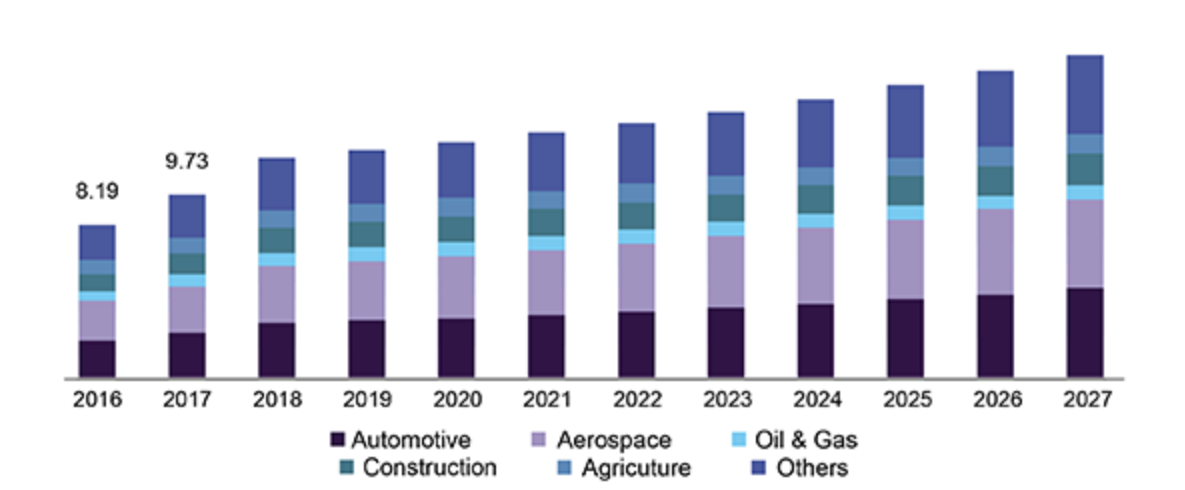
\includegraphics[width=0.6\textwidth]{./Images/Forgingindustry.png}
\caption{U.S. metal forging market size, 2016-2027 (USD Billion)}
\label{ForgingMarket}
\caption*{\textbf{Source}: www.grandviewresearch.com}
\end{figure}

Globally, the commercial segment represents around 51 \% of the aerospace industry in the United States, figure \ref{Forg2}, due to the fact that the demand for air passengers for Asia-Pacific travel is increasing over time. The second is the military segment, which is estimated to grow due to the increase of the defense budget, which remains one of the flags of this country\cite{market}.\par
Nowadays, the automotive and aerospace industries account for about 50\% of US production using forging techniques \footnote[]{These predictions were made before and during the appearance of the COVID-19 virus. Since the aerospace industry was one of the sectors most affected, they may not be up to date.\cite{hall2020beyond}},as we can see in figure \ref{ForgingMarket} \cite{market}.\par




\begin{figure}[h]
\centering
\includegraphics[width=0.6\textwidth]{./Images/Forg2.png}
\caption{Global aerospace forging market share, by aircraft, 2019 (\%)}
\label{Forg2}
\caption*{\textbf{Source}: www.grandviewresearch.com}
\end{figure}




\subsection{Forging Process}

Forging is a process that converts a metal in an object through compressive forces on a discrete part in a set of dies.
The process requires a few steps which depend on the complexity of the object to be produced.
Figure \ref{ForgingSteps1} is shown the generalized stages of typical forging process.

\begin{figure}[h]
\centering
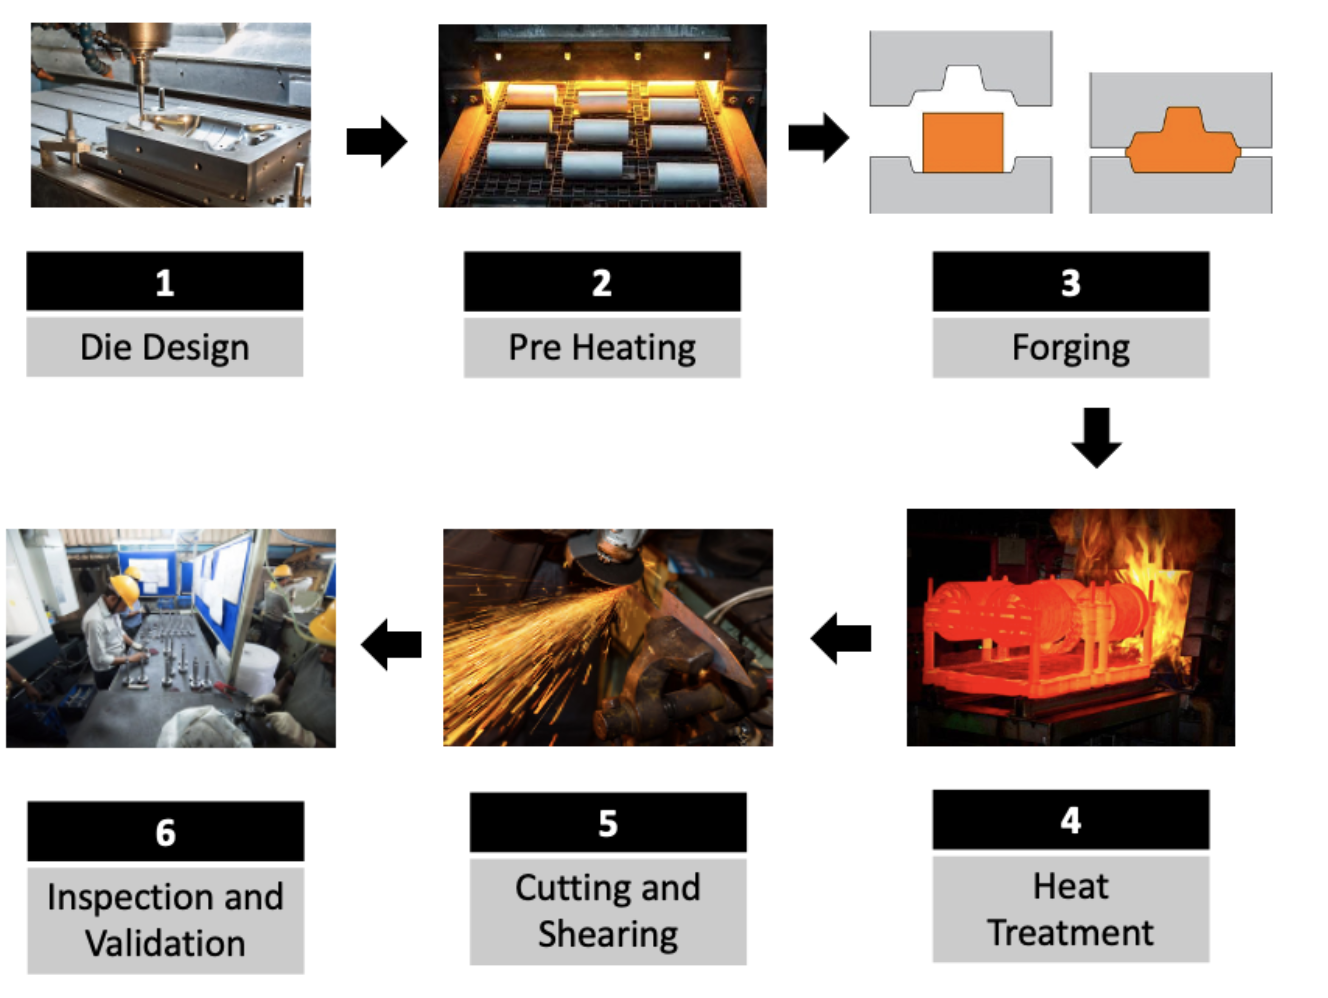
\includegraphics[width=0.7\textwidth]{./Images/ForgingSteps.png}
\caption{Generalized Forging Process}
\label{ForgingSteps1}
\end{figure}

\textbf{\emph{1. Die Design and Design of Forging Parameters}}\\

Die and mold manufacturing represents a significant area of production technology , the most restrictive aspect to be considered is the tools' cost. The construction of a metal stamping die requires a high number of resources and people, which will make the die building more expensive and, for this reason the bigger quantity of parts produced the more economically profitable it becomes \cite{souza2015estudo}.\par
The manufacture of a die and its ability to produce parts depends on several factors. The main areas of concern are:
\begin{itemize}
    \item \textbf{Parting Line} - The Parting Line is usually the central line, which separates the two dies. For a complex part, designing the parting line may not be a simple task \cite{site3,smith1990design}.
    \item \textbf{Flash and Gutter} - During the compression of the material against the die, the flash material can flow into a gutter. A good design can prevent an unnecessary increase of the forging load with excess flash \cite{site3,smith1990design}.
    \item \textbf{Draft Angles} - When designing the die, it is necessary to take into account the way the part will be removed from the die. Tilt angles are sometimes used to facilitate this removal \cite{site3,smith1990design}.
    \item \textbf{Fillet} - The fillet is a small radius provided at the corners to ensure smooth flow of metal into the matrix cavity. A small fillet leads to rapid wear of the die and an improper metal slip \cite{site3,smith1990design}.
    \item \textbf{Die material} - 
The die must be made of a hard material resistant not only to high temperatures but also resistant to mechanical and thermal shocks, as well as it should be a high resistance to wear \cite{site3,smith1990design}.
\end{itemize}



\vspace{50}


\textbf{ \emph{2. Pre Heating}}\\

Depending on the temperature at which the metal is forged, the forging can be classified as cold, warm or hot forging.\par
Cold forging involves forging with open die or close die and use of lubricant close to room temperature. Forgings of carbon steel and standard alloys are commonly cold forged, not requiring this production step. This type of forging offers an economically competitive advantage, since the forged part requires little finishing that normally makes the part more expensive\cite{site5,bryson2005heat}.\par
Warm forging is a type of forging that forges the part above the ambient temperature to below the recristallization temperature. Compared to cold forging, warm forging has the potential advantages of reduced tool loads, increased ductility, elimination of annealing needing before forging and favorable forging properties that can eliminate heat treatment\cite{site5,bryson2005heat}.\par
In hot forging, the metal and the die are heated to the same temperature. The objective of this step is to avoid hardening by deformation, in this way the metal is heated to the recrystallization temperature in such a way that the recrystallization occurs simultaneously with the plastic deformation\cite{site5,bryson2005heat}.\par
Hot forged components have greater ductility, which makes them desirable for many configurations. In addition, as a technique, hot forging is more flexible than cold forging, as customized parts can be manufactured\cite{site5,bryson2005heat}. \par
\vspace{5}


\textbf{\emph{2. Forging}}\\

During forging the metal is compressed under high pressure for a part to reach the desired shape. \par
In general, forging can be classified based on how metal flow is confined, as open die or closed die[14], figure \ref{OpenClosedDied}. \par


\begin{figure}[h]
  \centering
  \begin{minipage}[b]{0.4\textwidth}
    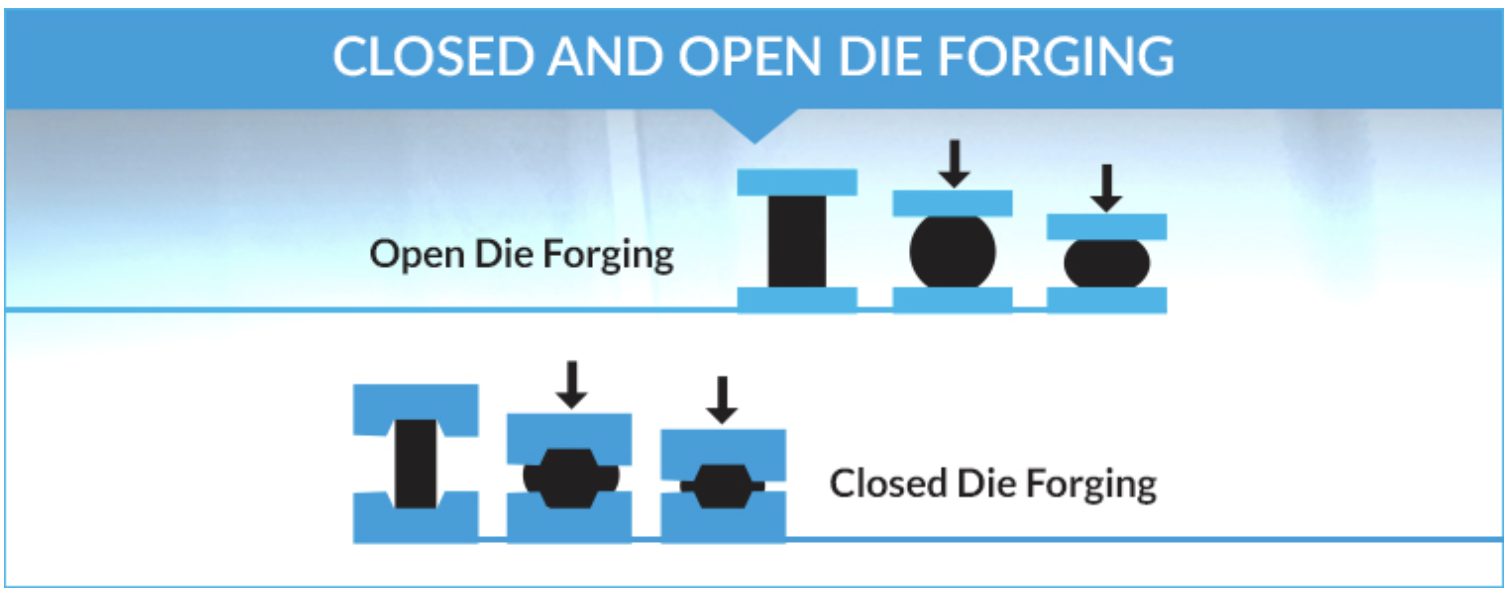
\includegraphics[width=\textwidth]{./Images/closedopen_die.png}
    \caption{Closed and Open Die Forging}
    \label{OpenClosedDied}
    \caption*{\textbf{Source:}www.indiaforging.com}
  \end{minipage}
  \hfill
  \begin{minipage}[b]{0.4\textwidth}
    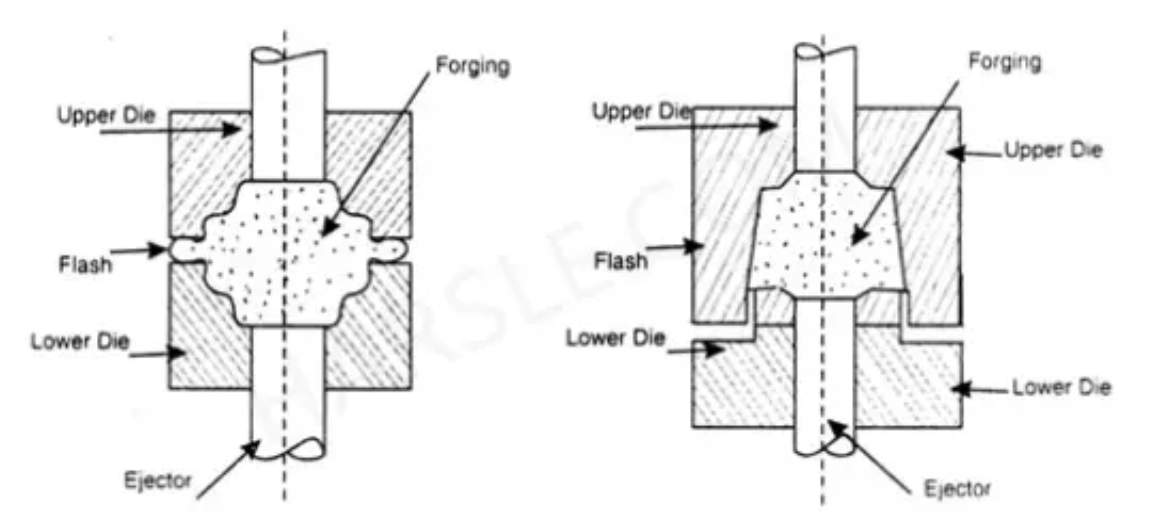
\includegraphics[width=\textwidth]{./Images/Flashless_die.png}
    \caption{Flash and Flashless Hot Forging}
    \label{Flashforging}
    \caption*{\textbf{Source:}www.harsle.com}
  \end{minipage}
\end{figure}

Forging is the molding of metal by plastic deformation. This process covers a multitude of equipment and techniques.
We can classify forging by:
\begin{itemize}
    \item Forging temperature - Hot, Warm or Cold Forging
    \item Die shape - Open Die Forging or Close Die Dorging
    \item Compressive forces - Drop Forging, Press Forging or Rolling Forging
\end{itemize}

Regarding the temperature and the type of die, it has been analyzed previously.\par
A far as of the shape of the die is concerned, forging can be classified as open die forging or close die forging.\par
Open die forging is performed using two flat dies, which are not normally touched, or which allows the material to be released freely in the lateral direction. This type of forging is used for large parts or discs, blocks or bars.\cite{site4,site3,souza2015estudo}\par
In closed die forging or  impression-die, the cavity is formed by using two or more dies which the metal is deforming undergoes plastic deformation through the pressure exerted \cite{site4} \cite{site3,souza2015estudo}.\par
Forging is a method of handling the metal to achieve the final product. Usually the design of this product is in a die, where the metal is pressed against it to obtain the desired shape. This metal manipulation is usually done using two methods: Drop forging or press forging. \par
A closed die can also be selected as flash or flashless, \textif{c.f.} figure \ref{Flashforging}. The flashless forging allows excess material not to escape through the concavity, while the flash type can occur \cite{site4,site3,souza2015estudo}.\par
The advantage of this forging is that it allows more complex shapes and closer tolerances than forging in the open die. Limit your ability to produce parts in great detail, or forging prevalent in the metallurgical industry\cite{site5,souza2015estudo}.\par

In the Drop Forging, forge hammers are used to deform the metal through several impact strikes on the metal surface \cite{site3,altan2004cold}. During the process the surface layers of the metal are manipulated in shape. However, the central area of the metal will remain relatively deformed. In this process, the deformation rate is difficult to control and generally the cost of this product is generally lower, for low production volumes, when compared to press forging \cite{site3,altan2004cold}.  \pair

In the press forging a slower and continuous pressure speed is used. The material is shaped evenly, from the surface to the center, making it an advantage over drop forging, as it allows for a stronger and more perfect final product\cite{site3,altan2004cold}.  \pair
In this process, the initial costs are much higher than using a hammer, making it more economical with increasing production volume. Despite being a longer technique, another advantage is a more controlled deformation rate that allows a stronger product\cite{site3,altan2004cold}. \par

Roll forging consists of two horizontal cylindrical rollers that form a round or flat bar. This type of forging is used to increase the length or decrease the thickness of the metal bar. This bar is heated and then passed through two rollers that contain patterned grooves and is progressively shaped as it is rolled by the machine \cite{site3}.\par
\vspace{20}
\textbf{ \emph{3. Heat Treatment}}\\

Heat treatment can be defined as controlled heating or cooling of metals made with a change in physical and mechanical properties.\par
In many cases, as metal parts go through different temperatures during a heating phase, going through heating and cooling cycles, thus altering some physical and mechanical characteristics of parts, with the possibility of having thermally affected parts zones \cite{bryson2005heat,souza2015estudo}. \par
However, heat treatment can be used for different purposes: to increase the material's resistance and/or to decrease the excess duration, allowing better machining and restoring ductility after an intense cold machining process \cite{bryson2005heat,souza2015estudo}. \par
The figure \ref{HTsteps}, it helps to understand how the heat treatment takes place.

\begin{figure}[h]
\centering
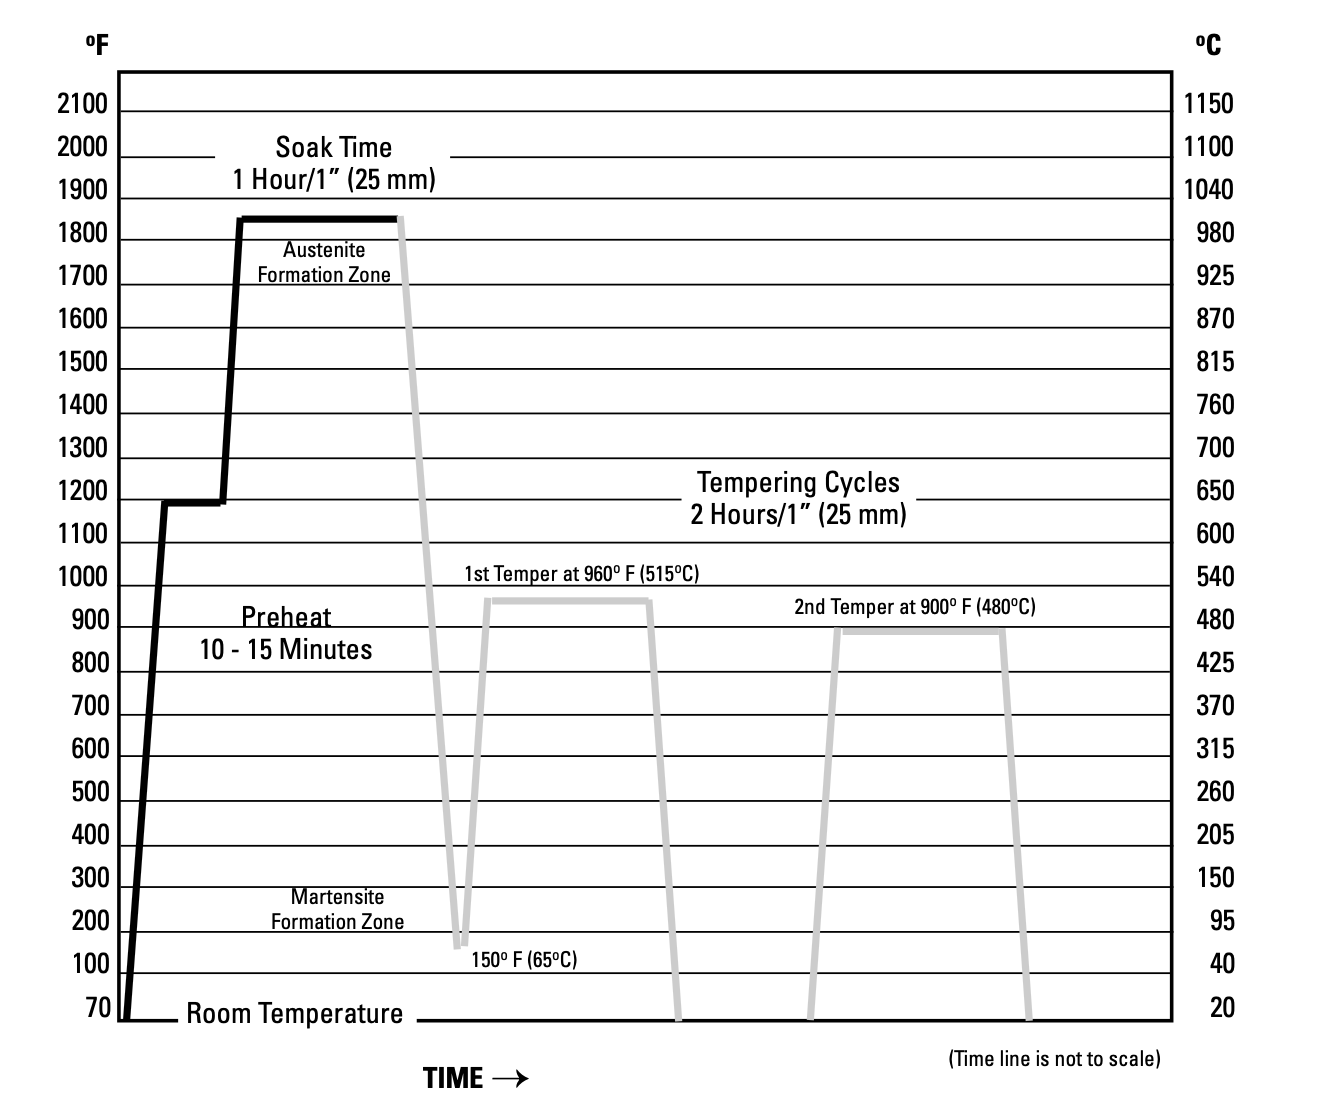
\includegraphics[width=0.6\textwidth]{./Images/HotTreat.png}
\caption{Generalized Hot Treatment Steps}
\label{HTsteps}
\caption*{\textbf{Source:} Heat treatment, selection, and application of tool steels \cite{bryson2005heat}}
\end{figure}

Depending on the application of the forged part, the residence times in the oven and the temperature at which the part must be raised are defined.
The main heat treatments used in forged metals are Annealing, Normalization, Stress Relief, Queching and Tempering.

\emph{Complete annealing} is a very general term that consists of heating the part above the critical zone and letting it cool slowly. Annealing will produce a more refined microstructure, in order to soften the metal to better withstand the constant pressures that the metal may undergo during the machining process \cite{huang2006hardening}. For this reason, this heat treatment is often used not only as a finishing process but also as a preheat use before machining. \cite{bryson2005heat,souza2015estudo}

\emph{Normalization} is a technique used to offer uniformity in grain size to the piece's metal. When normalized, the piece is heated to a temperature just above the critical point, keeping enough time to form smaller and more uniform metal grains. After heating above the critical point, the part is cooled in the open air until it reaches room temperature.
 This transformation is called grain refinement, which takes the piece to become more uniform, but above all improving the strength and toughness of the material.\cite{bryson2005heat,souza2015estudo}
 
\emph{Stress relief} is a technique for removing internal stress from a metal. These stresses can be caused many times by the process of cold machining or non-uniform cooling. Stress relief consists of reheating the metal below the critical temperature and then uniformly cooling the part.\cite{bryson2005heat}

\emph{Quenching} involves rapidly cooling the material after heating it above the critical region. After being quickly cooled, the alloy turns into martensite, a hard and brittle crystalline structure. For this reason, after Quenching, tempering is normally used.\cite{bryson2005heat,souza2015estudo}
\emph{Tempering}
Martensite steel is very hard but very brittle. Tempering is the heat treatment that seeks to offer a better combination of hardness, strength and toughness.
Tempering is effective in relieving tensions caused by cooling, in addition to decreasing hardness for specific intervals.\cite{bryson2005heat,souza2015estudo}
In this process, the metal is reheated to a relatively low temperature with a controlled time to produce the desired final requirements for the part.

\vspace{50}

\textbf{ \emph{4. Cutting and Shearing}}\\


\textbf{\emph{Wire Electric Discharge Machining}}\par 
\vspace{5}\par
Wire \ac{EDM} is a machining process that emerged in the 1960s with the aim of manufacturing hardened steel die \cite{el2018fundamentals}. It is a non-traditional machining process widely used in today's manufacturing. It involves removing metal using an electric discharge wire machining the part with high speed and accuracy \cite{tominaga1987electrode,rajurkar2013review}.\par 
This relatively recent technology is commonly used for machining hard materials that are difficult to work with conventional forging. The process consists of immersing a part in a dielectric which use a cutting wire powered electrically that cuts the metal, \textif{c.f.} figure \ref{EDM} \cite{rajurkar2013review}. First, machines used a \ac{NC} and nowadays they use \ac{CNC}. \par
This technology has brought several benefits, since it allows the cutting of very hard materials without them being subjected to excessive pressure from the impact used in machining. It also allows achieving high design tolerances \cite{el2018fundamentals}.\par

\vspace{10}

\textbf{\emph{Multi Axis Mills}}
\vspace{5}\par
\ac{MM} is a process that involves a tool that moves in 3, 4 or 5 directions depending on the type of machine. This machine,\textit{c.f.} figure \ref{MM}, allows the milling of excess material with a water jet or laser cut \cite{el2018fundamentals}.\par
In the most recent machines, a CAD is used through computer software that will allow the machine to know where to cut. This technology allows a better finish of the piece for more complex pieces, and the detail of them can be increased \cite{son2009hybrid}.\par
Since the machines are using a software witch give a precise indications of cutting the part, then this can be replicated hundreds of times and each product will be exactly the same, in addition to needing only a supervision of it.\par
\vspace{5}


\begin{figure}[h]
  \centering
  \begin{minipage}[b]{0.45\textwidth}
    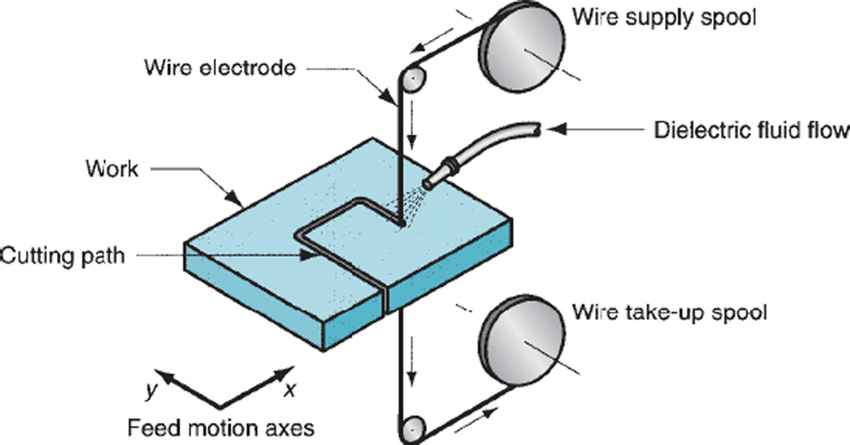
\includegraphics[width=\textwidth]{./Images/EDM.png}
    \caption{EDM Cutting Process}
    \label{EDM}
    \caption*{\textbf{Source:} Comprehensive materials finishing \cite{saleh20171} }
  \end{minipage}
  \hfill
  \begin{minipage}[b]{0.3\textwidth}
    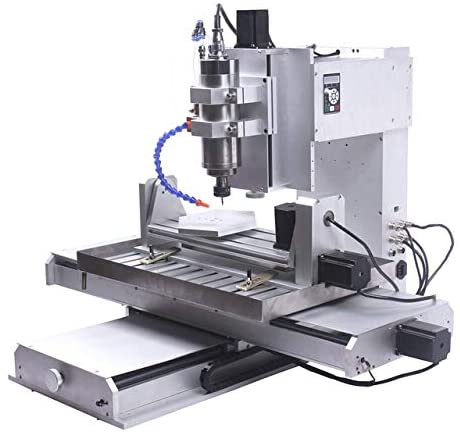
\includegraphics[width=\textwidth]{./Images/MM.png}
    \caption{A 5-axis Multi Axis Machine and a part manufactured with it.}
    \label{MM}
    \caption*{\textbf{Source:} www.wardjet.com}
  \end{minipage}
\end{figure}

\vspace{10}
\textbf{\emph{Thermochemical Treatment}}\par
\vspace{10}
This treatment aims to change the surface properties of the metal. In general, materials with high hardness have a high resistance to wear, but low toughness and resistance to impact.\par
In some parts, a tough core and a wear-resistant surface are desired. For this reason, low carbon steels are subjected to thermochemical treatment by carburizing, which increases the carbon content on the surface, increasing its resistance to wear, while preserving the properties of the core.The means to carry out the treatment are carbon or nitrogen sources which can be in the form of solids, liquids or gases \cite{czerwinski2012thermochemical}.\par
The process consists of combining repeated heating and cooling, keeping the material in contact with C or N, such as specific salts, oils or gases for that purpose \cite{czerwinski2012thermochemical}.\par
\vspace{5}
\textbf{\emph{Grinder}}
\vspace{5}

Grinding is an important metal machining process. The process allows for a finer finish and increases the useful life of the part \cite{el2018fundamentals,malkin1984grinding}.
With the interaction of abrasive grains on the surface of the part, metal removal occurs \ref{grinder2}. This removal occurs by a shearing process in which it normally involves a rotating wheel with abrasive particles on the metal surface, firgure \textit{c.f.} \ref{grinder1} \cite{el2018fundamentals,malkin1984grinding}. Several machines are used in this process as:
\begin{itemize}
    \item Whetstone;
    \item Power tools such as angle grinders;
    \item Bench grinders.
\end{itemize}

The process today can be used through an axis machine, such as Multi Axis Mills, in which it uses \ac{CNC}.

\begin{figure}[h]
  \centering
  \begin{minipage}[b]{0.4\textwidth}
    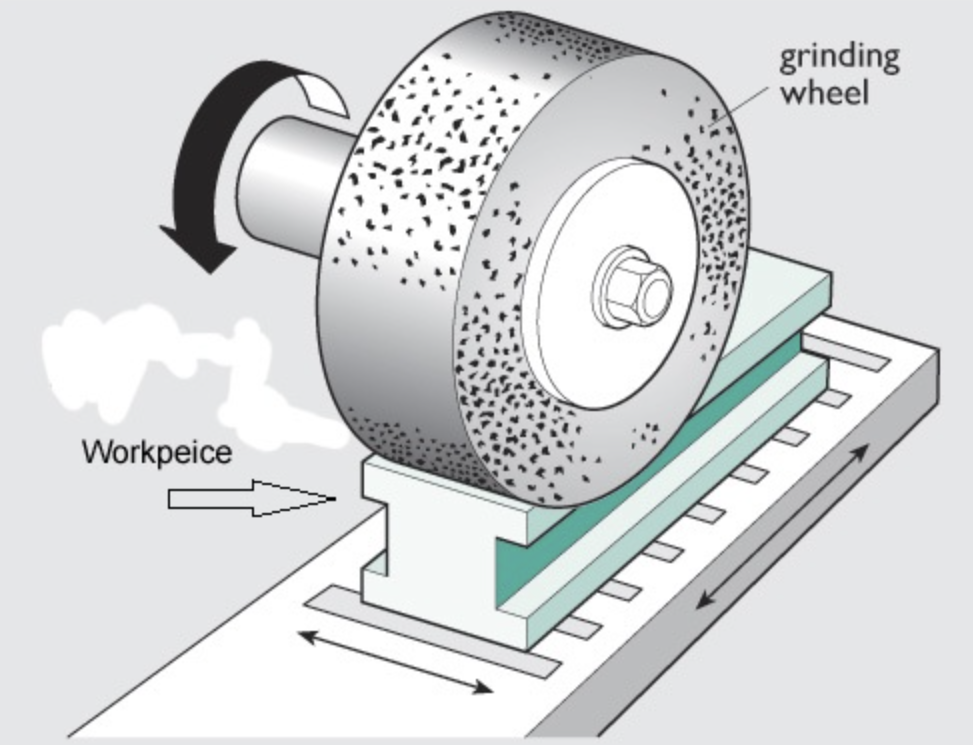
\includegraphics[width=\textwidth]{./Images/GW.png}
    \caption{Grinder Rotating Wheel}
    \label{grinder1}
    \caption*{\textbf{Source:} www.surfacegrindingmachine.wordpress.com}
  \end{minipage}
  \hfill
  \begin{minipage}[b]{0.45\textwidth}
    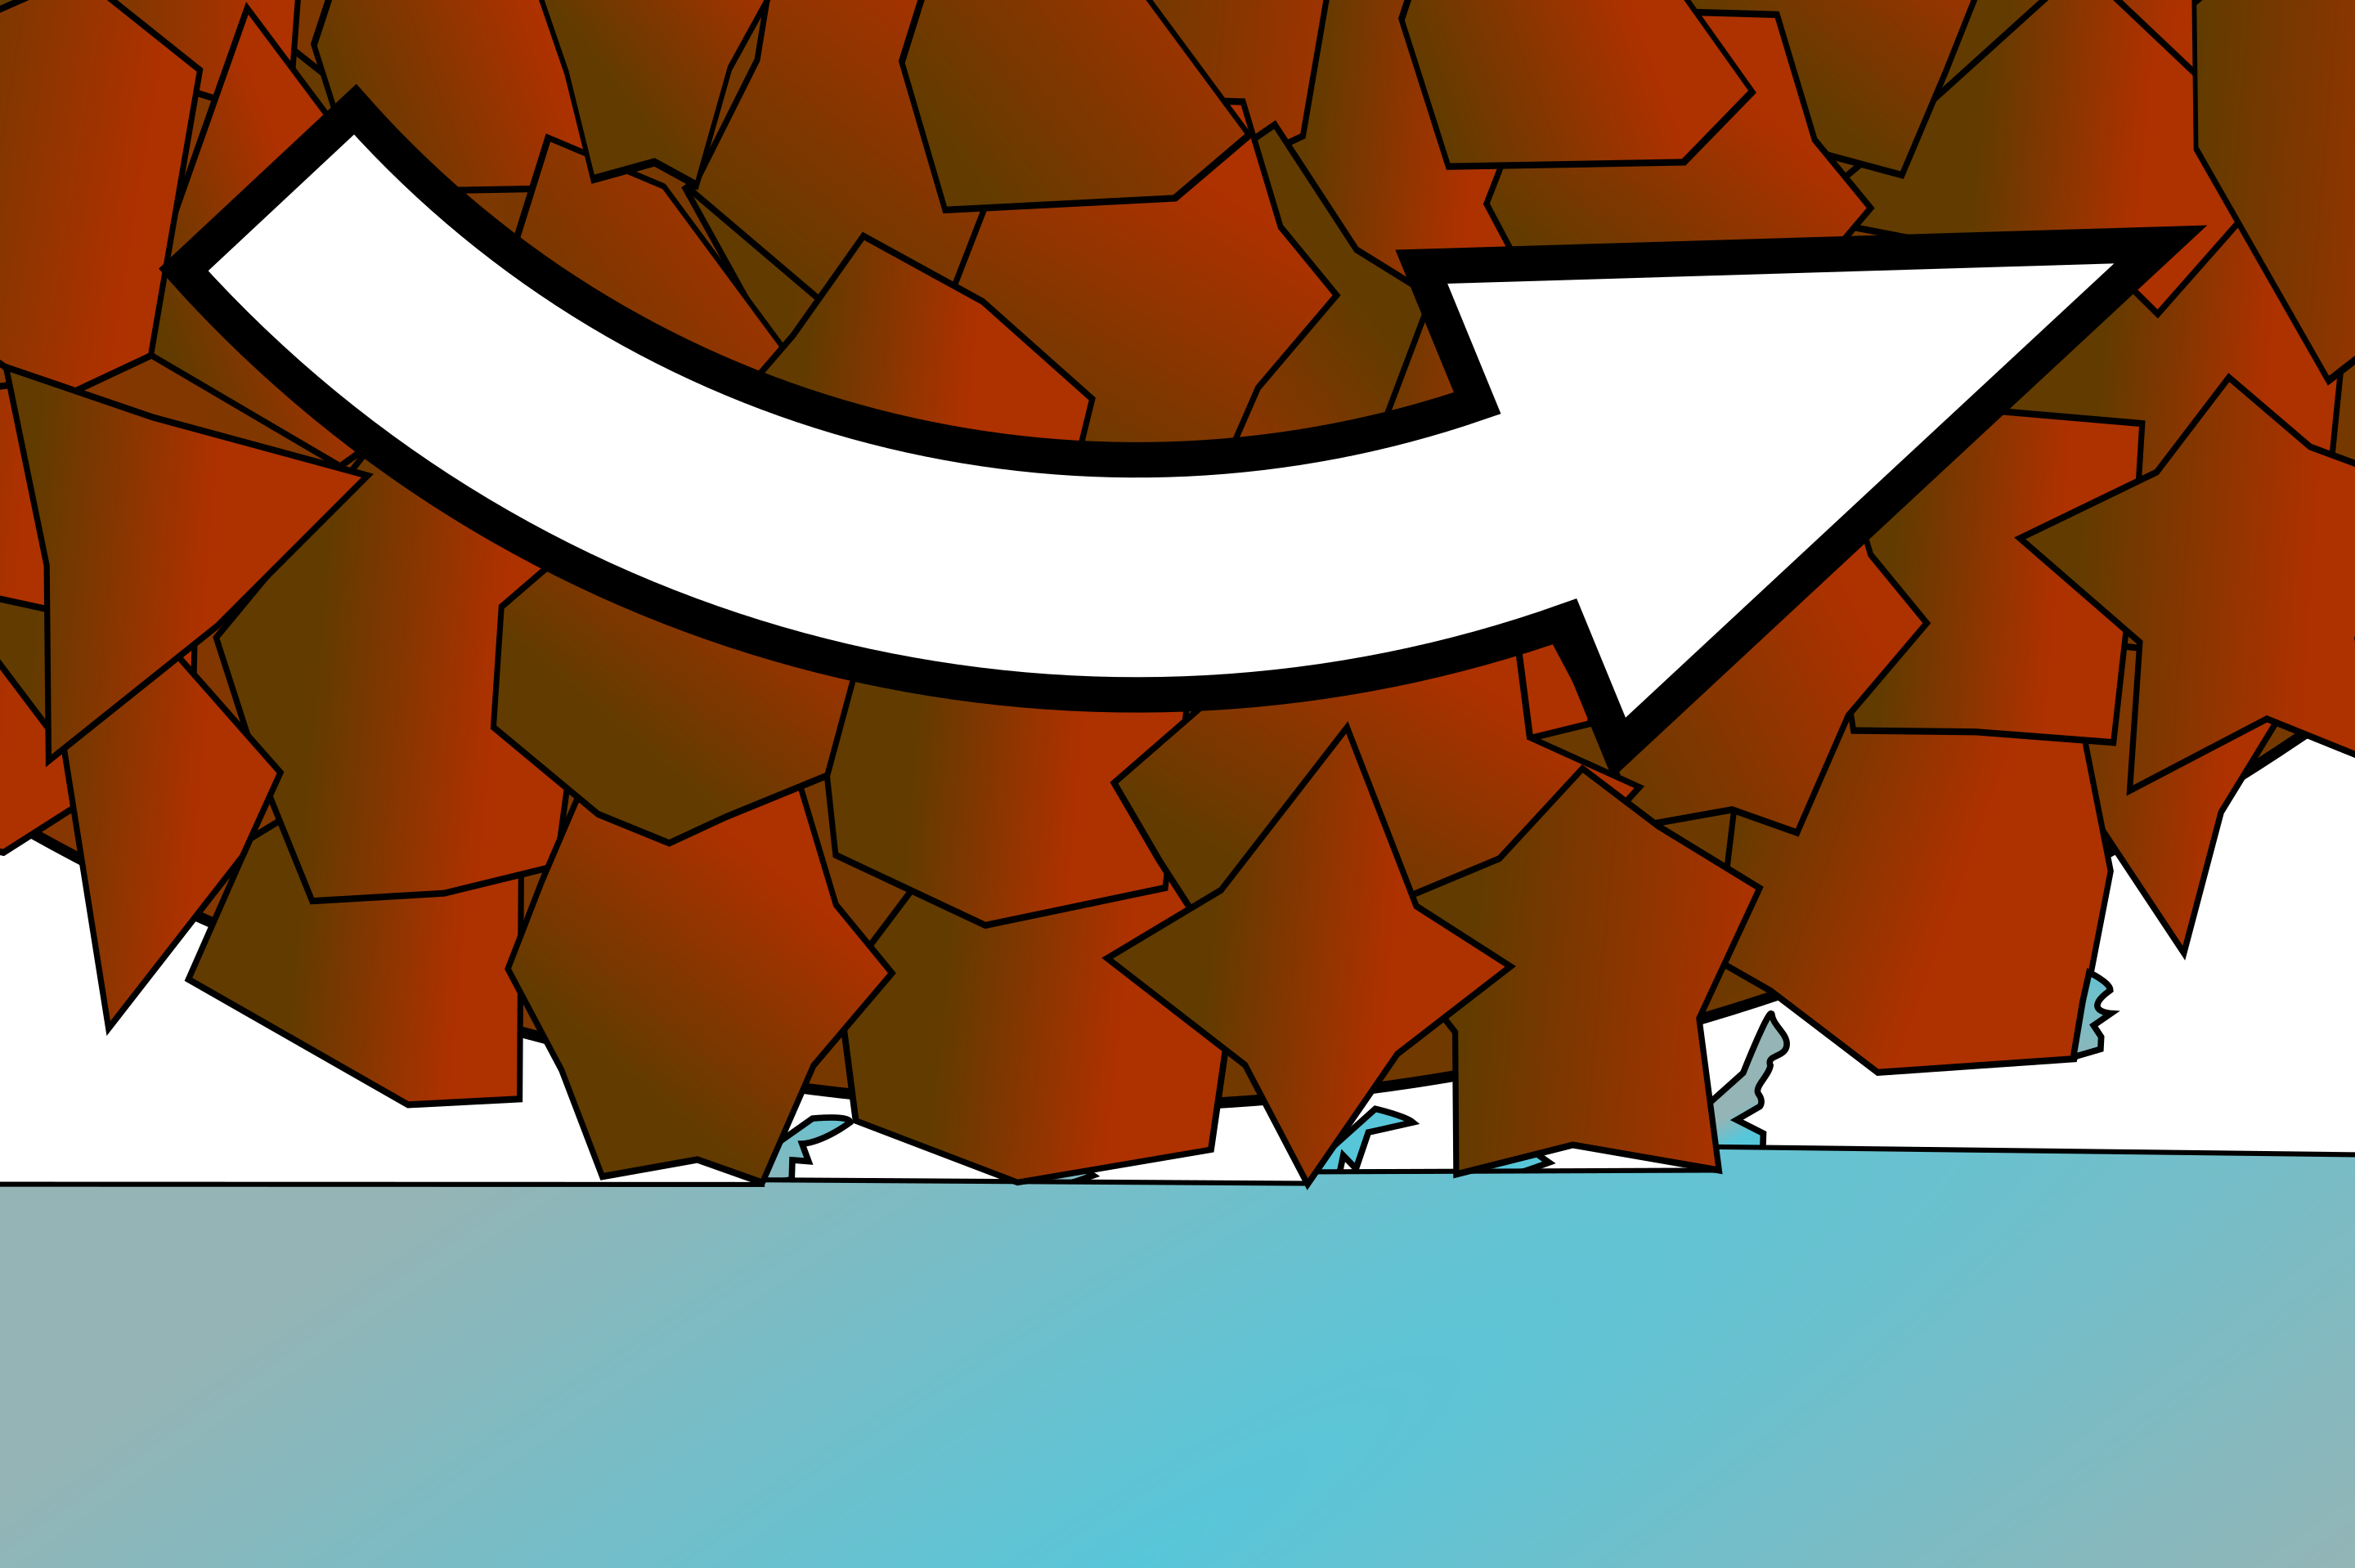
\includegraphics[width=\textwidth]{./Images/grinder2.png}
    \caption{Abrasive Process in Grinder}
    \label{grinder2}
    \caption*{\textbf{Source:} www.wikipedia.org/grinder}
  \end{minipage}
\end{figure}



\pagebreak

% #############################################################################
\section{AM Technology}

\subsection{Introduction}
Additive Manufacturing, also called 3D Printing, is a relatively recent method of manufacturing parts from \ac{CAD} file. In contrast to subtractive manufacturing methods, such as forging, AM generally builds the part layer by layer.\par
A computer-developed project is exported to the \ac{STL} file format that is read by the equipment AM that build it. \par
Nowadays, AM can produce parts using any type of raw material, from plastics, metals, ceramics to composites. There are several techniques available that can be classified according to their raw material: powder base, liquid base and solid base.\\

\subsection{History}

\begin{figure}[h]
\centering
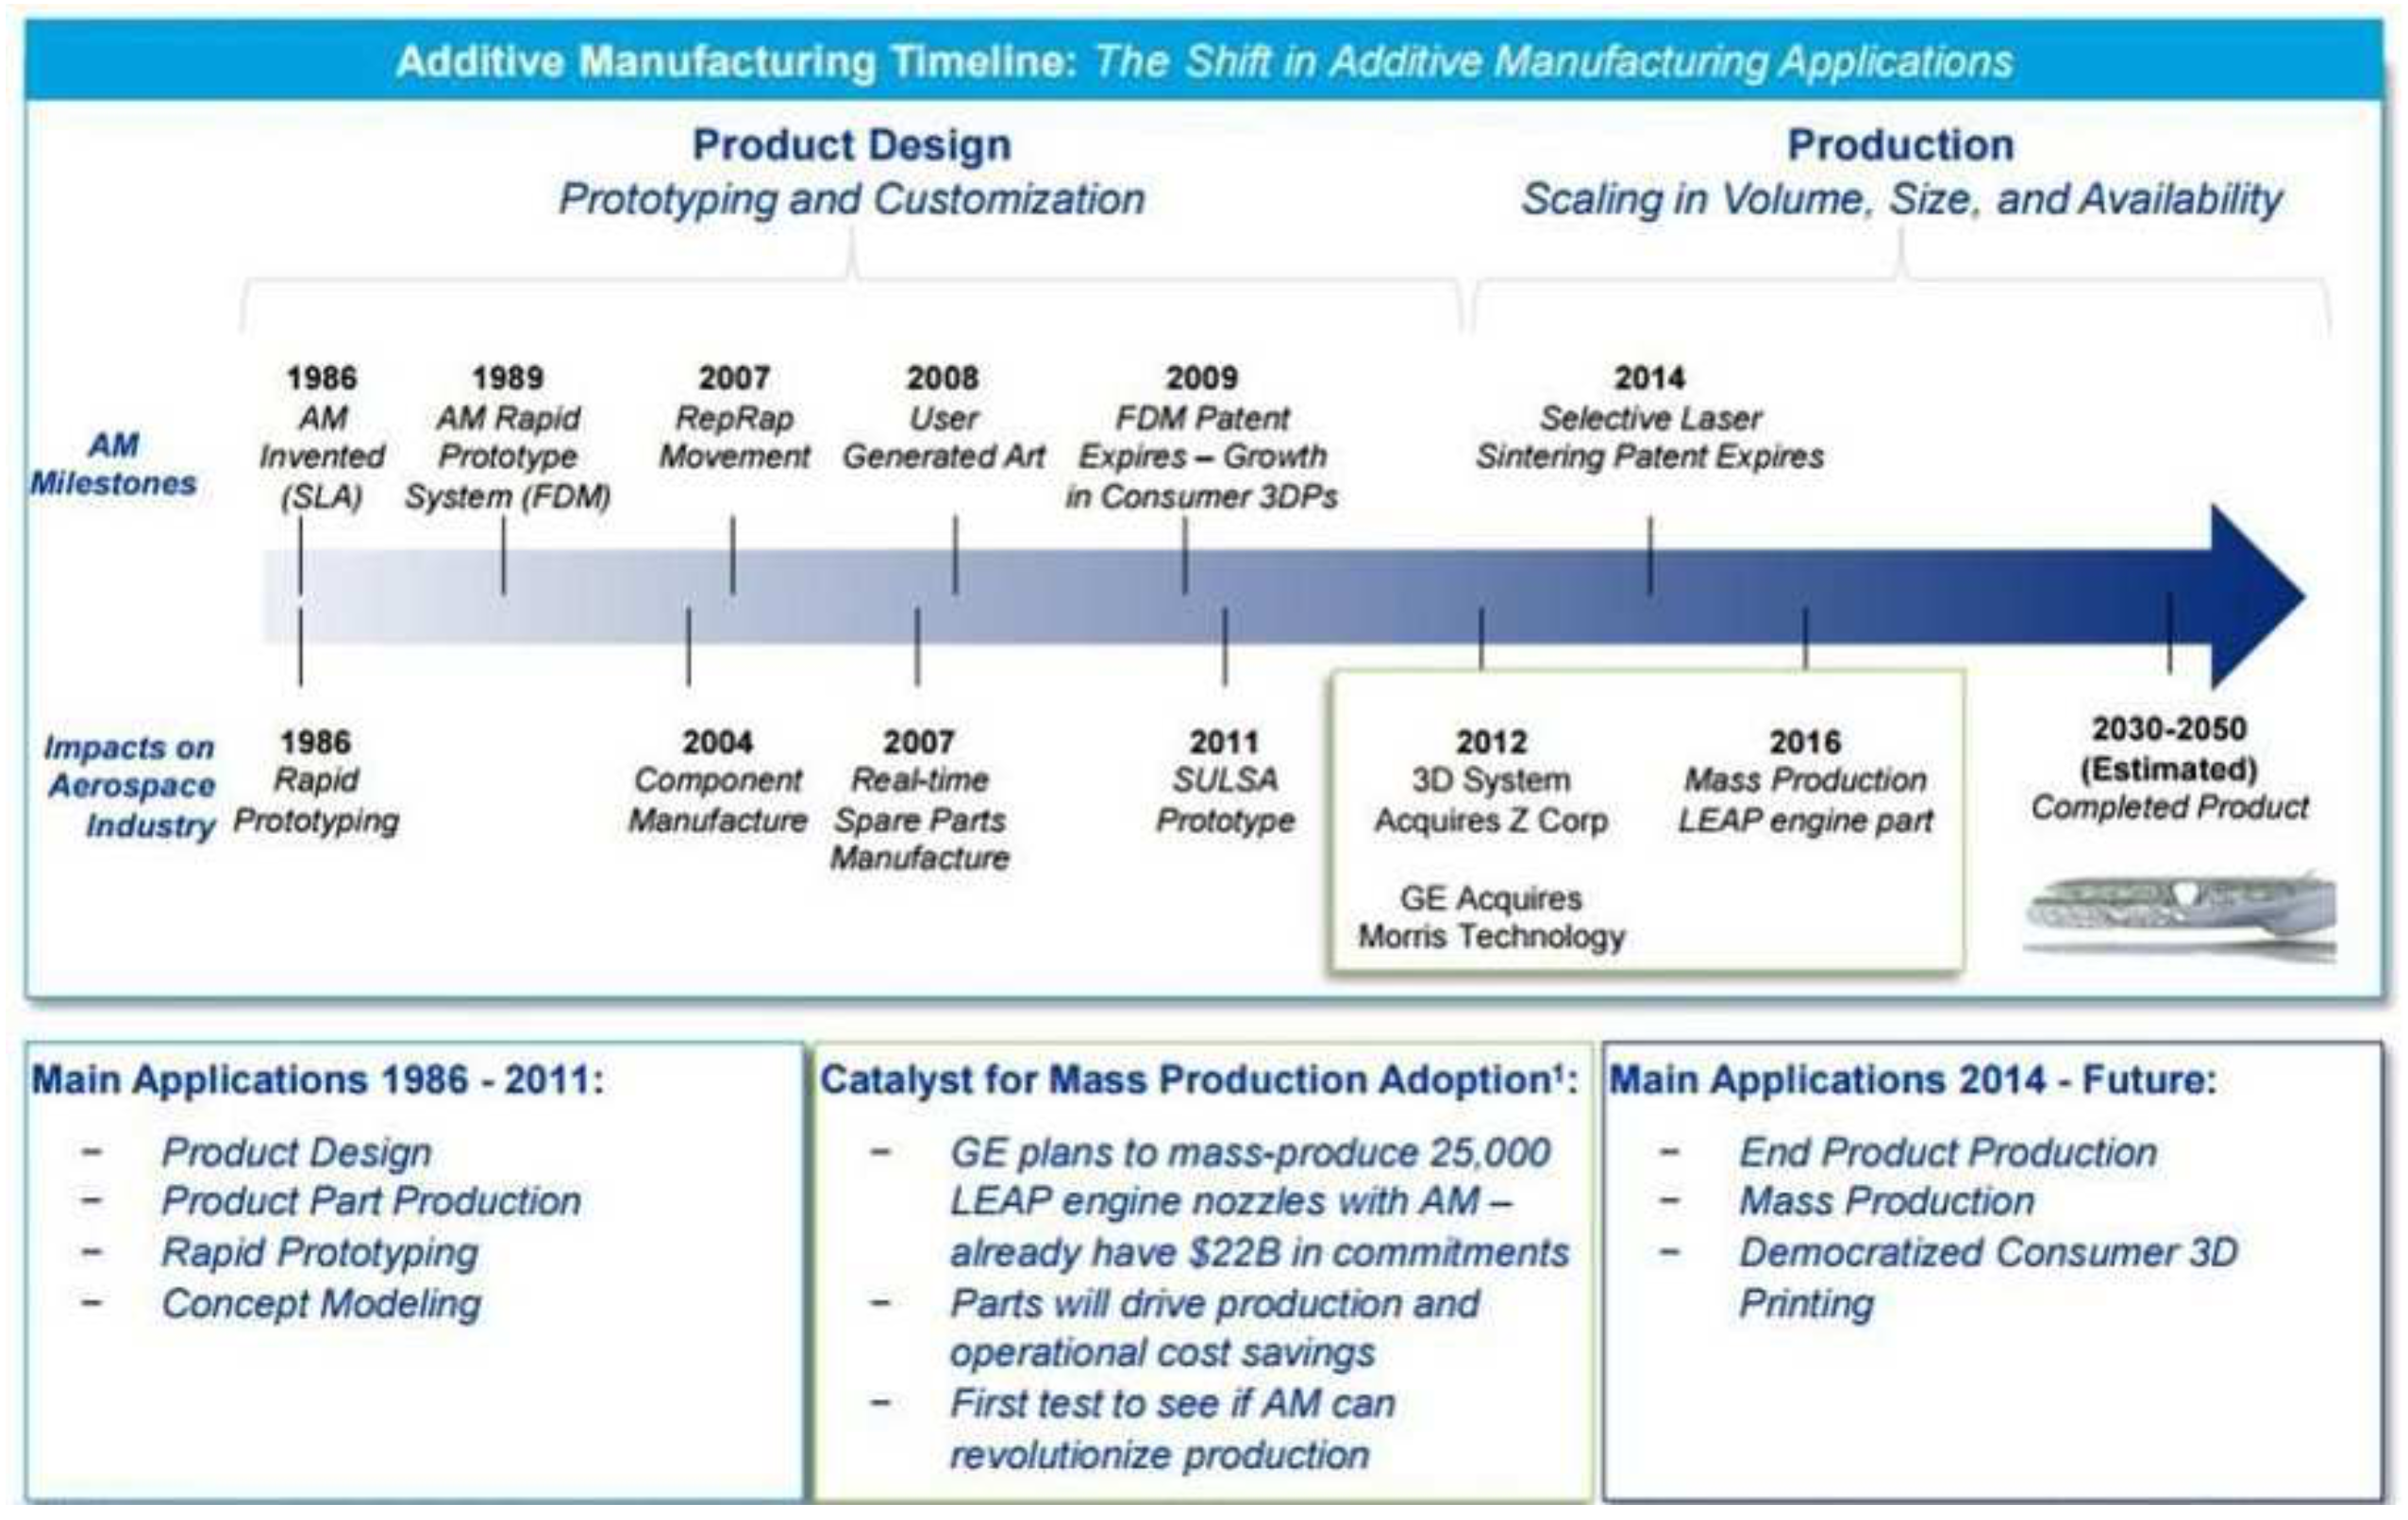
\includegraphics[width=0.8\textwidth]{./Images/AM_HISTORY}
\caption{AM important milestones}
\caption*{
\textbf{Source:} Additive manufacturing paths to performance, innova-tion, and growth\cite{cotteleer20143d}}
\label{AMHist}
\end{figure}
Additive manufacturing is defined as "the process of joining materials to make parts from 3D model data, usually by layer in combination with subtractive manufacturing"\cite{lee2017fundamentals}.
Over the years, AM has taken important steps, essentially in product design, as represented in the figure \ref{AMHist}.
The first steps of AM were in the 1980's, where parts called Rapid Prototyping were developed in a quick way to check their shape, fit and function\cite{bartolo2011history,bourell2016perspectives,wohlers2014history}.\par
In 1987, the company 3D systems developed a plastic processing system known as stereolithografy. This process consists of solidifying thin layers of polymer using a laser UV. Since then, many companies researched and made progresses in order to develop new technologies, improve process and commercialize them. \cite{bourell2016perspectives,wohlers2014history}\par
In the 90's, the bet of several companies allowed the development of other techniques based on polymers such as, \ac{FDM}, \ac{SGC},  \ac{LOM} and  \ac{SLS}.\cite{bourell2016perspectives,wohlers2014history}\par
In addition to the new AM techniques, processes based on Metals were initially introduced through laser sintering and only later by powder sintering.\cite{bourell2016perspectives,wohlers2014history}\par

The improvement of computers, CAD software also had a development that came to revolutionize the process, causing AM to take off exponentially in the mid 2000's. The internet had a strong influence on this growth by promoting global interaction.\cite{wohlers2014history}\par
Until the mid-2000's, AM was only possible as plastic softs as the prototyping goal. Since then, with the range of materials increasing sharply, it is possible to create new parts, strongers with more details and more functional characteristics.\cite{wohlers2014history}\par
The manufactured process is currently applied to almost all market areas, from electronics, aerospace and automobiles to education and medicine.
In the aerospace industry, AM has the potential to change the future of aircraft manufacturing, from design to construction.\par
The main aircraft manufacturers are already producing parts with AM although they are still non-critical parts and to a limited extention.\par 
Aircraft manufacturers strive to reduce the weight of aircraft and the use of AM can assist in this weight reduction \cite{birtchnell2013freight}.\par
Airbus has already adopted this technology. It changed internal components like brackets or cable routing cards from a conventional manufacturing process to 3D printing on its A350 \cite{warwick20153}.\par
Boeing applied 3D thermoplastic printing for prototypes and components for use on its 737,747,777 and 787 aircraft.\cite{walton20146th}
Some authors believe that the results of AM in this industry are livable and that in the near future we can have an aircraft almost 100\% manufactured with AM \cite{walton20146th}\cite{coykendall20143d}. However, not everyone agrees that AM will be able to overcome the efficiency and agility of the global freight industry.\par


\subsection{AM Processing Steps}

AM requires some steps of multiple difficulties depending on piece's complexity.\par
The process begins with the creation of a CAD model using a computer software or scanning an existing object. The software slices the CAD and creates a file with instructions for the machine.The machine creates the object layer by layer by forming each layer via the selective placement.After the Build Process is completed, the object is carefully cleaned and it may have to go through finishing processes, \textit{c.f.} figure \ref{Aviao}.\par

\begin{figure}[h]
\centering
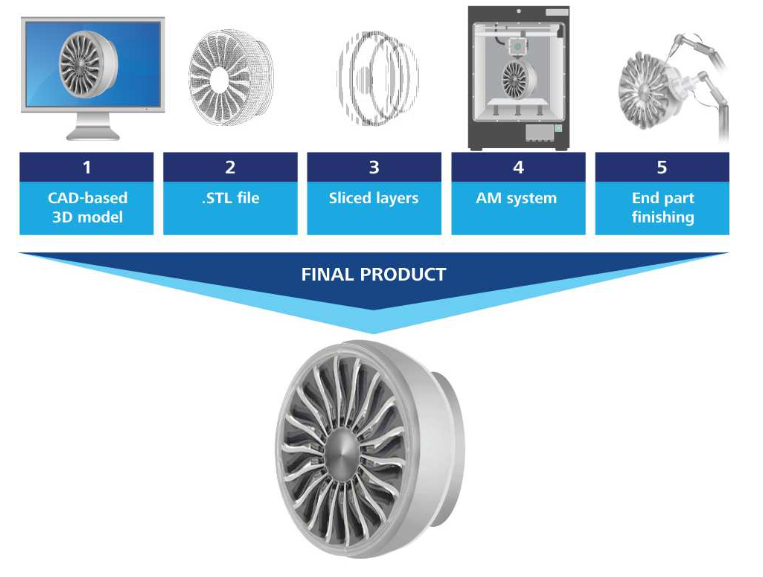
\includegraphics[width=0.5\textwidth]{./Images/AM_STEPS.png}
\caption{Generalized AM process}
\label{Aviao}
\caption*{\textbf{Source:}Cost estimation model for the directed energy deposition process adopting an activity-based approach \cite{santos2018cost}}
\end{figure}


\subsubsection{Modelling}
The\ac{AM} process must start with a 3D model using CAD software that must contain a precise internal and external description of the object.
This file will have to be converted to a language compatible with AM machines \cite{gibson2014additive}.\par
There are several file formats, the most used are \ac{STL} and \ac{AMF}.
STL transforms a simple model like a square box, where its surfaces can be approximated with twelve triangles. The most complex is the surface, the more triangles are produced. While the \ac{AMF} is a file format that allows for more details such as colors, materials and constellations\cite{gibson2014additive}.
Finally, with the specialized software's help, the file is divided into several transversal layers creating a new STI file, as shown in the figure \ref{STL}\cite{gibson2014additive}.
In this last point, there are some aspects to be considered such as the orientation of the piece, supports and support structure.

\begin{figure}[h]
\centering
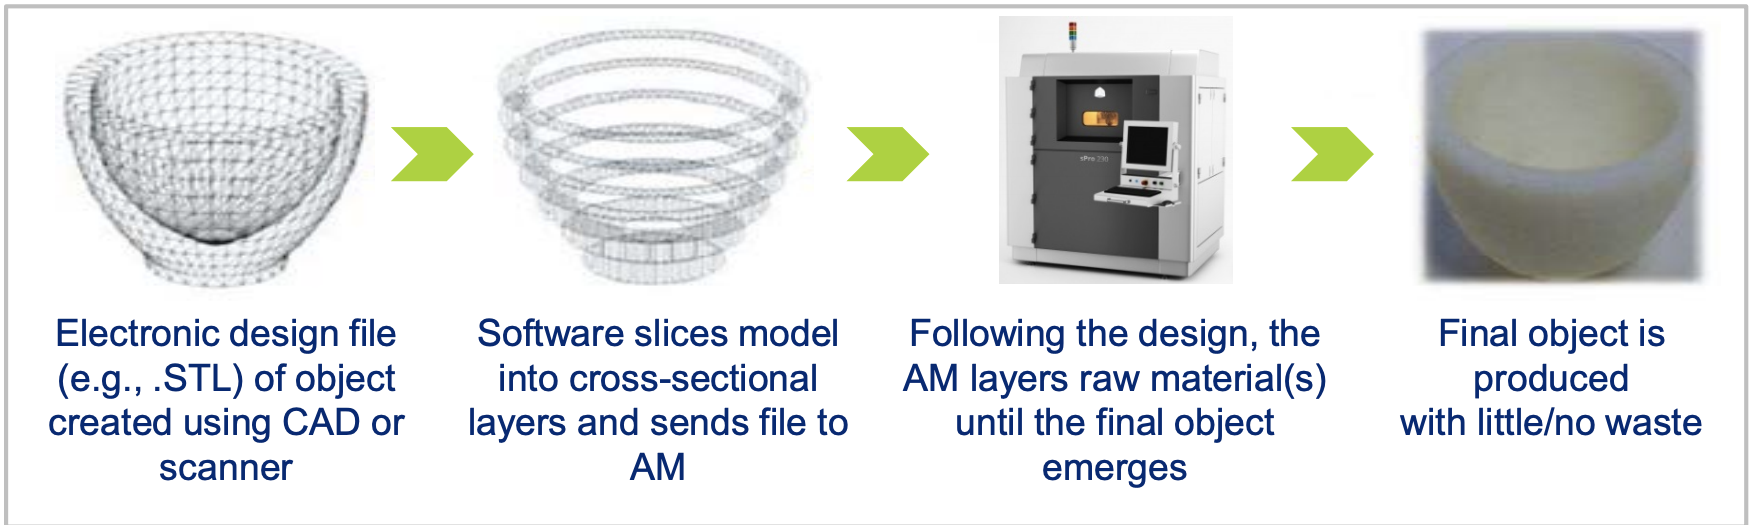
\includegraphics[width=0.5\textwidth]{./Images/STL.png}
\caption{Modelling Stages}
\label{STL}
\caption*{\textbf{Source:}Additive manufacturing paths to performance, innovation, and growth \cite{cotteleer20143d}}
\end{figure}



\subsubsection{Additive Manufaturing technologies}

This is the main stage of the whole process, after the AM machine receives the file, the part can then be produced.\par
First, the operator must configure the machine by preparing the raw material and determine the process parameters. Then the part's construction is in charge of the AM machine, which is an automated task that requires only the operator's supervision.\par
Additive manufacturing is, as the name itself implies, the process that adds material during the production of a part. For which, different technologies are used and regarding the technologies applied to metal parts, we can classify them in 4 main categories: \ac{MJ}, \ac{BJ}, \ac{PBF} and \ac{DED}.

\vspace{10}

\textbf{\emph{Material Jetting}}\par
\vspace{10}

\ac{MJ} is a 3D printing process more like conventional 2D printers. In the \ac{MJ}, a print head distributes droplets of a photosensitive material that solidifies under ultraviolet light, forming a layer\cite{lboro}. The material used in this technology is thermoset photopolymers in liquid form, figure \ref{MJ}.\par
Steps of the \ac{MJ} printing process:
\begin{enumerate}
    \item The resin is heated to 30-60C to achieve an ideal viscosity\cite{3dhubs}.
    \item The print head travels on the platform and deposits droplets at designated locations\cite{3dhubs}.
    \item A UV light source fixed to the print head cures the deposited material, solidifying it. Thus, it gives rise to the first layer of the piece\cite{3dhubs}.
    \item After the construction of the first layer, the platform goes down one layer height and the process is repeated until the entire piece is completed\cite{3dhubs}.
\end{enumerate}
\ac{MJ} is classified as a technology capable of producing smooth parts with surfaces compared to injection molding, with a high dimensional precision (more or less 0.1\%)\cite{3dhubs,lboro}. However, MJ parts are mainly purchased for prototypes not issued due to their poor mechanical properties. MJ is an expensive technology making it unviable for some applications\cite{lboro,3dhubs}.

\begin{figure}[h]
\centering
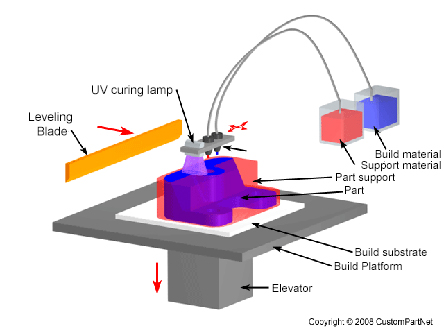
\includegraphics[width=0.6\textwidth]{./Images/MJ.jpg}
\caption{Material Jetting}
\label{MJ}
\caption*{\textbf{Source:} www.lboro.ac.uk}
\end{figure}
\\
\vspace{10}
\textbf{\emph{Binder Jetting}}\par
\vspace{10}
The Jet Binder is a multi-stage AM process developed by MIT in the early 1990s\cite{gokuldoss2017additive}.
This 3D printing process uses a powder-based material and a binder. An impression involves several processes:
\begin{enumerate}
    \item The powder material is spread on the construction platform using a roller \cite{lboro2}.
    \item The print head deposits the bonding adhesive on the powder, when necessary \cite{lboro2}.
    \item The construction platform is lowered by the layer thickness of the model \cite{lboro2}.
    \item Another layer of dust is spread over the previous layer. The object is formed where the powder binds to the liquid \cite{lboro2}.
    \item Dust not attached to the position around the object \cite{lboro2}.
    \item The process is repeated until the entire object is made\cite{lboro2}.
\end{enumerate}

\ac{BJ} allows a wide variety of colors and allows the use of raw materials such as metals, polymers and ceramics.
However, due to the use of binder, the parts are not suitable for structural parts. \cite{ziaee2019binder,gokuldoss2017additive}.

\begin{figure}[h]
\centering
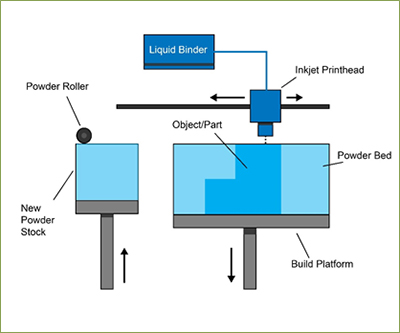
\includegraphics[width=0.4\textwidth]{./Images/BinderJet.jpg}
\caption{Binder Jet\\
Source: https://www.lboro.ac.uk/}
\label{}
\end{figure}

\vspace{50}
\textbf{\emph{Powder Bed Fusion}}\\
\vspace{5}
\ac{PBF} methods use an electro or laser beam to melt and melt the metal powder.In the figure \ref{PBF} we can see a schematic of a \ac{PBF} machine. Building a part with \ac{PBF} has the following steps:
\begin{enumerate}
    \item A layer of metallic powder is spread on the platform.
    \item A laser melts the first layer
    \item A new layer of powder is spread on the previous layer using a roller.
    \item More layers are spread, fused and added
    \item The process is repeated until the entire model is created.
\end{enumerate}

This process has several techniques for melting metal powder such as: DMLS, EDM, SHS, SLM and SLS.\par

DMLS, was developed by Germany's EOS. This printing technique fuses very thin layers of metallic powder using a yb fiber laser beam. The system operates in a protective atmosphere of nitrogen and argon allowing the use of a wide range of metals. \cite{udroiu2012powder}\par
DMLS has an excellent and precise resolution in the creation of its objects, being used for the construction of prototypes of instruments, instruments and objects for the use of the aeronautical and space industry. \cite{3dilla}\par
EDM developed by the Swedish company Arcam, builds the pieces layer by layer by melting the metallic powder through an electron beam. When electrons reach the metallic powder at high speed, the kinetic energy is converted into thermal energy by melting the metallic powder. \cite{udroiu2012powder}\par
The high quality of finish allows this process to become standard for medical applications and parts construction for aircraft \cite{lboropbf}.
SHS uses a heated thermal printing head to melt the powder material. The use of this thermal head and not a laser permanent the necessary electrical energy. The process is used for prototypes not to use. \cite{lboropbf}\par

SLM uses a high-power iterbium fiber laser to fuse or metallic powder\cite{udroiu2012powder}.  A roller or blade is used to spread the powder, which is then melted by the laser, building the piece in layers. It is a relatively fast process that requires the use of an inert gas and has high energy costs \cite{lboropbf}.\par
This technique is used for dental application, turbine blade with internal shaped cooling channels, vane segment for aerospace applications. \cite{udroiu2012powder}\par
SLS and SLM have the same principle, differing only in that the SLM achieves a complete fusion of the powder layers and the SLS does not \cite{wagner2016additive}. The SLS process benefits from having no additional support structure and from some machines monitoring the temperature of layers by automatically adapting the laser power. The models have a cooling period to guarantee a high tolerance and quality of fusion. \cite{lboropbf}
\begin{figure}[h]
\centering
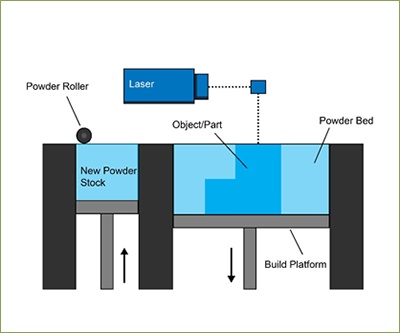
\includegraphics[width=0.4\textwidth]{./Images/PBF.jpg}
\caption{Powder Bed Fusion Machine}
\label{PBF}
\caption*{\textbf{Source:} www.lboro.ac.uk}
\end{figure}
\\

\\ \textbf{\emph{Directed Energy Deposition}}\\
\par
DED is a collection of processes that uses thermal energy, laser or electron beam, focused on melting and bonding materials in the form of powder or wire\cite{shamsaei2015overview}.\par
The process can be used with polymers, ceramics but it is with metals that DED together with GMP, are more reliable and used AM techniques.
Almost all weldable metals can be printed with DED. This includes titanium and its alloys, inconel, tantelo, aluminum, etc\cite{bourell2017materials,shamsaei2015overview}.\par
A typical DED machine consists of a nozzle mounted on a multi-axis arm, which moves in 4 or 5 directions, which deposits the material by melting on the specific surface where it solidifies. \par
DED consists in the following steps\cite{DED2}:
\begin{enumerate}
    \item The arm with the nozzle moves on the printing platform.
    \item The material is deposited by the spout on the platform's surface.
    \item The material is supplied in the form of wire or powder.
    \item The material is melted using a laser or electron source after deposition.
    \item More layers are added until the object is finished.
\end{enumerate}

DED presents itself as a fast and inexpensive AM technology compared to the others. However, fusion processes require more research and improvement of fusion processes and require post-processing to achieve the desired effect\cite{DED}.

\begin{figure}[h]
\centering
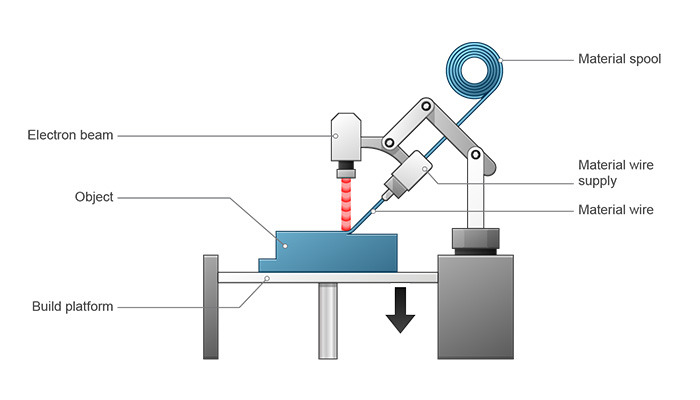
\includegraphics[width=0.6\textwidth]{./Images/DED.jpg}
\caption{DED\\
Source: \cite{DED2}}
\label{DED}
\end{figure}
\\

\subsubsection{Finishing Process}
 
 \textbf{\emph{ Shot Peening}}\\

 
 Shot peening is a cold working process used in the aerospace and automotive industries \cite{meo2003finite}.\par
Surface treatment procedures such as grinding, milling, bending or heat treatment procedures cause residual tensile stress. This Residual Tensile Effort leads to a reduction in the life cycles of the parts. Shotpeening converts Residual Tensile Stress into Residual Compression Stress, which allows to increase the complication of the service life and as maximum load resources of the parts.\cite{majzoobi2005three}\par

The process is used for better resist once to metals' fatigue. It consists of bombarding small hardened spheres, usually steel, against a surface of the object creating small plastic deformations on the part's surface, causing changes in the mechanical properties. \cite{majzoobi2005three,meo2003finite}\par
The impact of each shot particle on the object generates a compression stress on the surface of the piece. A surface notched by the ball generates a compaction force below the notch. Hammering generates not only one but severals notches on the surface, forming a layer of residual compaction stress on the part. \cite{meo2003finite,SP}\par
The creation of the residual compression stress created on the part's surface helps to prevent the appearance of cracks as they cannot propagate in the compression environment generated by hammering. \cite{meo2003finite,SP}\par

\begin{figure}[h]
  \centering
  \begin{minipage}[b]{0.4\textwidth}
    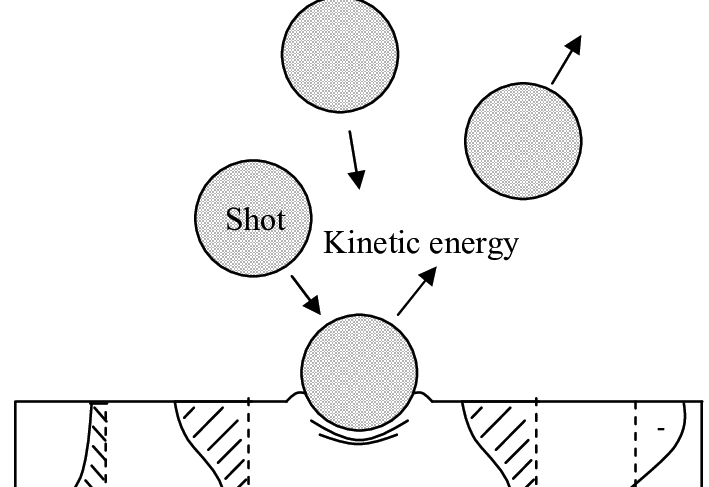
\includegraphics[width=\textwidth]{./Images/sp1.png}
    \caption{Compression Stress}
    \label{grinder1}
    \caption*{\textbf{Source:} Texture Gradients in Shot Peened \cite{maawad2010texture}}
  \end{minipage}
  \hfill
  \begin{minipage}[b]{0.4\textwidth}
    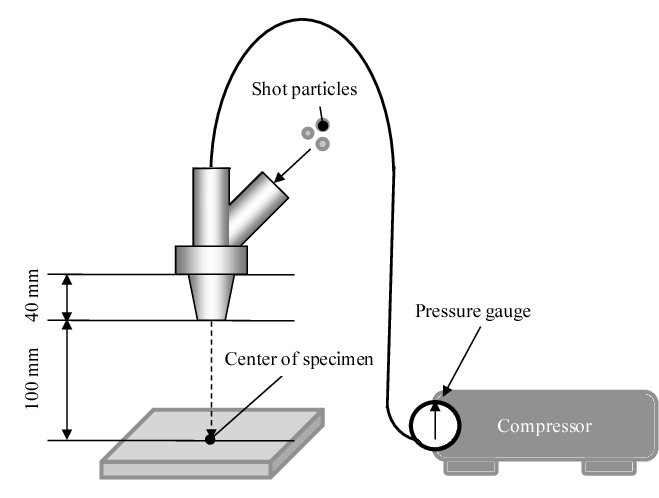
\includegraphics[width=\textwidth]{./Images/sp.png}
    \caption{Shot Peening Machine}
    \label{grinder2}
    \caption*{\textbf{Source:} Modelling  of  particle  behaviour  in  shot  peening  process \cite{kato2014modelling}}
  \end{minipage}
\end{figure}

\vspace{20}
 \textbf{\emph{Hot Isostatic Pressing}}\\


\ac{HIP} is a post processing used to reduce porosity of metals and increase the density of ceramic materials.
The process consists of placing the object in a chamber where it is pressed on all sides with equal pressure (isostatic pressure) and with an elevated temperature for consolidation in a dense solid\cite{atkinson2000fundamental}. \ac{HIP} applies high temperatures from several hundred to 2000\degree C and isostatic pressure from several tens to 200MPa at the same time. Argon gas is the most used pressure medium. The gas at 1000\degree C and under pressure 98MPa can cause an intense convection due to the low density, viscosity coe and high thermal expansion coe\cite{HIP}.\par
Through \ac{HIP} it is possible to obtain material formats not very different from the initial one after high pressures, contrary to what happens with hot press, see in the figure\ref{hip1}\ref{hip2}. \cite{atkinson2000fundamental}.
\ac{HIP} is used in a wide range of fields:
\begin{itemize}
    \item Pressure powder sintering;
    \item Diffusion connection of different types of materials;
    \item Removal of residual pores in sintered items;
    \item Removing internal defects in castings;
    \item Rejuvenation of parts damaged by fatigue or creep;
    \item High pressure impregnated carbonization method.
\end{itemize}




\begin{figure}[h]
  \centering
  \begin{minipage}[b]{0.3\textwidth}
    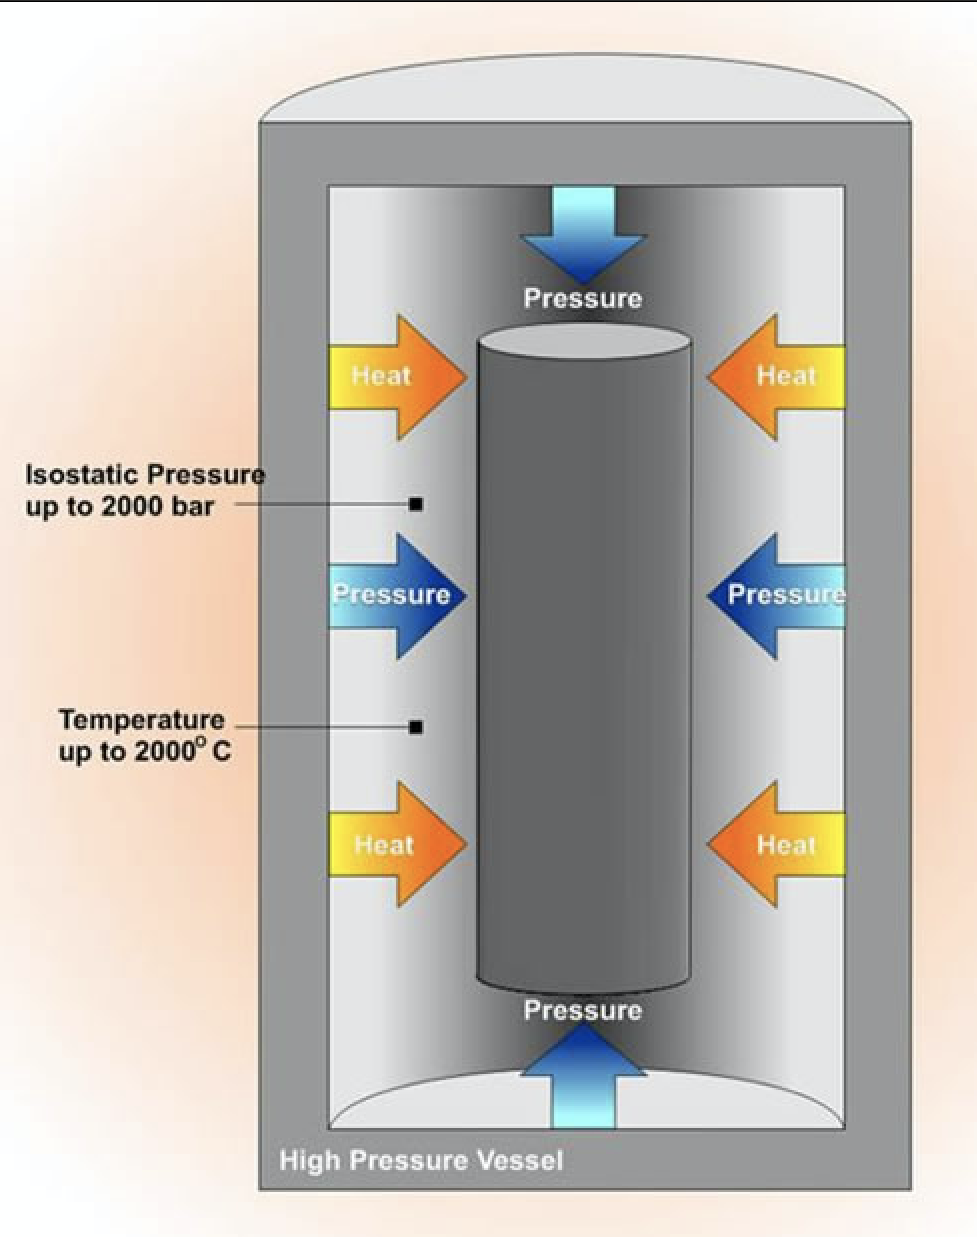
\includegraphics[width=\textwidth]{./Images/hp1.png}
    \caption{HIP process}
    \label{hip1}
    \caption*{\textbf{Source:} www.azom.com}
  \end{minipage}
  \hfill
  \begin{minipage}[b]{0.5\textwidth}
    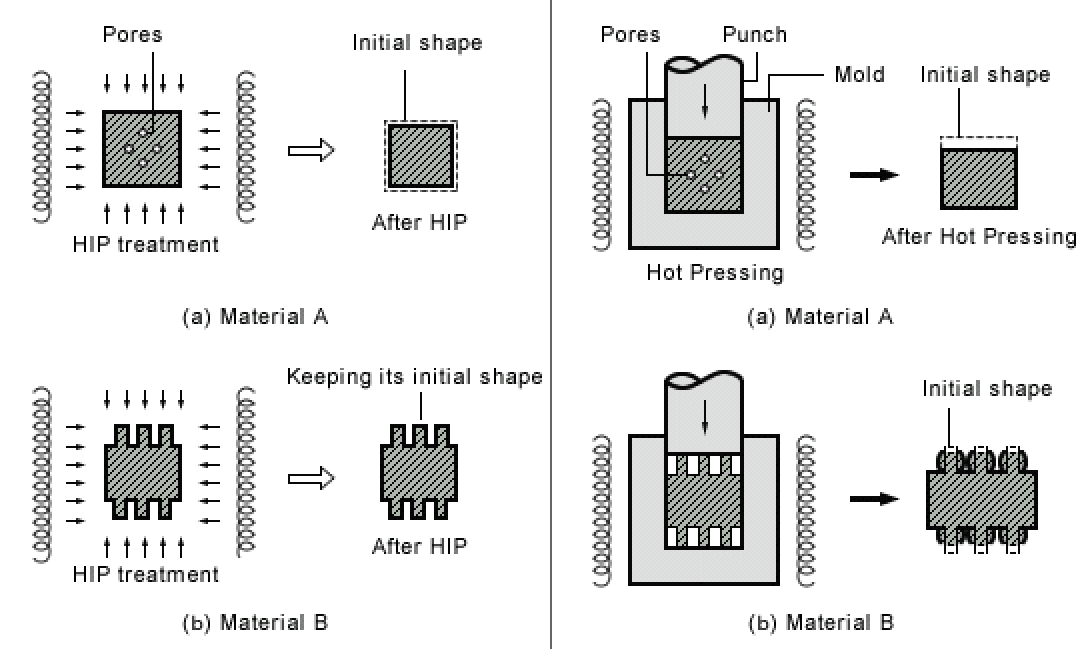
\includegraphics[width=\textwidth]{./Images/hp2.png}
    \caption{HIP vs conventional compression}
    \label{hip2}
        \caption*{\textbf{Source:} www.kobelco.co.jp}
  \end{minipage}
\end{figure}



\section{Capabilities and Challenges of Additive Manufacturing and Forging}

Additive Manufacturing is widely adopted in many industrial sectors, particularly in the aeronautical sector. The main companies in the world are converting to this technology but not leaving the forging part in the production of their parts. It is important to note the main differences and limitations of the technologies:\\
\vspace{20}\\
 \textbf{\emph{Strengh}}: Although \ac{AM} already works with a wide variety of raw materials, its results still have a high degree of uncertainty. Therefore, its use is limited to parts that provide little mechanical effort, since deposited layers can create weakened parts if they are not perfectly calibrated\cite{AMD}. The total density of AM metal parts is not possible without the subsequent \ac{HIP}. On the other hand, forging is a well-known technique, widely used and reliable, with the properties of the materials already tabulated. Deposited layers can create weakened parts if they are not calibrated perfectly
 \vspace{20} \\
 \textbf{\emph{Design Complexity}}: Parts with more complex geometries and internal cavities are a limitation of conventional forging. With conventional techniques it is difficult to produce objects with a high complexity and detail and sometimes they have to be subdivided into several less complex parts, which subsequently without connections forming an original piece\cite{he2007transport}.
With the tools of advanced software and AM brought the possibility to produce uniform parts with complex changes geometries and high internal and external resolution\cite{toyserkani2004laser}.
 \vspace{20}\\
 \textbf{\emph{Part Size }}: AM has restrictions on the size of the parts. The size of the objects is limited to the size of the machine's printing chamber. Producing large chambers for AM machines is expensive, since inert atmospheres or vacuums are required. On the other hand, AM allows you to produce very small parts with high detail\cite{saboori2017overview}.
With forging there is no limitation on the parts's size, it is necessary to adapt only the size and strength of the hammers and presses, as well as the EDM and Multi Axis Mills cutting machines. Compared to the production of micro parts, they lose detail as they become smaller\cite{saboori2017overview}\cite{frazier2014metal}.
 \vspace{20}\\
  \textbf{\emph{Timings}}: The 3D impression of a product compared to forging has a significant reduction in time if we think about all stages of production. Engineers can create a prototype with AM immediately after its design - so you can be tested as its properties and not wait weeks or months for a traditionally manufactured prototype to arrive.\cite{AMPC}\par
  On the other hand, for higher production volumes, conventional manufacturing mechanisms are still the fastest choice, at least until AM printers become better and faster.
 \cite{attaran2017rise}
  
 \vspace{20}\\
 \textbf{\emph{Weight Parts}}: AM it became possible to produce weight with complex structures compared to forging without compromising some of its properties. What becomes a great advantage for some industrial sectors like an Aerospace that looks for the lightest parts to improve fuel efficiency \cite{huang2016energy}.
 \vspace{20}\\


 \textbf{\emph{Tooling}}: The comparison of 3D printing for the traditional manufacture of electronic components, researched in Italy found out that 93.5\% of the cost of manufacturing a product using the traditional method is linked to tools. \cite{boubekri2015economics}
A strong advantage of additive manufacturing is the ability to significantly reduce or eliminate the use of tools.
 \vspace{20}\\
 \textbf{\emph{Material Waste}}: Traditional methods such as forging generate a significant amount of waste. However, with AM, only the amount of raw material needed to produce a product is used.
Thus reducing waste with 3D printing will also have a positive impact on the environment. \cite{boubekri2015economics}
 \vspace{20}\\
 \textbf{\emph{Manufacturing}}:
In a conventional metohd the production of the pieces is done in several places and then stored, after which they can be distributed when necessary. With AM, parts are produced simultaneously in the same production and in the same place. It allows the possibility of reducing inventories, as it is possible to produce parts in remote locations on demand, eliminating large warehouses of stocks and the need for transportation \cite{tofail2018additive}\cite{pereira2019comparison}.
 \vspace{20}\\
 \textbf{\emph{Cost Prodution}}: 3D printing offers a good solution for manufacturing small quantities. Forging requires a large investment in die and custom tools not being economically profitable for low demands \cite{boubekri2015economics}.
On the other hand, additive manufacturing does not offer economies of scale. \cite{boubekri2015economics}
 \vspace{20}\\
 \textbf{\emph{Produts Quality }}:AM technologies still have some quality limitations in terms of tensile stresses and in terms of construction resolution in same technology cases, with significant surface roughness. In contrast, forging is a much more studied method with reliable and known results\cite{tofail2018additive}.
 \vspace{20}\\
  \textbf{\emph{Finishing Equipment}}: The parts produced with AM when compared with the parts produced with conventional method have greater roughness and purity, forcing the post-processing \cite{AMD}. To eliminate the roughness characteristic of AM technology, surface treatment using the grinder or shot peening is necessary. For parts produced using powder, they have purity that will have to be treated with a hot isostatic press that will reduce the purity and increase the part's resistance \cite{loh1992overview}. Particularity of \ac{PBF}, is the use of supports in printing that after printing have to be separated from the part that can be removed with a water bath if they are soluble or cut using cutting tools if they are insoluble in water.\par
 \vspace{20}
 
 \noindent
  \textbf{\emph{Raw Materials}} - Currently, additively manufactured parts still have little variety of materials available. Despite the constant innovation and research in this new technology, the truth is that the raw materials associated with it are still scarce \cite{herzog2016additive}. Forging on the other hand has a greater variety of raw materials available.\par
 

\newpage
\section{Costs Modelling}
 
 \vspace{20}\\

Over the years, mass production factories have been migrating to developing countries such as China and India. Large American and European companies have been forced to rapidly shift production to lower volumes of innovative and sustainable products with high added value. Due to the need of greater flexibility and low-cost volume production, manufacturers have been looking for tools and new techniques. One of the emerging techniques is additive manufacturing. AM allows for freedom of design, removal of tool requirements and good profitability for low economic volumes. \cite{mellor2014additive}\par
Comparison conventional manufacturing methods with AM has been a constant issue on companies and production engineers. 3D printing of metallic hair combined with the part's redesign has a positive impact on cost savings. \cite{atzeni2012economics}\par
There are three ways to assess the costs of additive manufacturing:
\begin{itemize}
    \item The first is to study under what circumstances AM is competitive in relation to traditional methods \cite{thomas2014costs}. In this analysis, it is not only important to assess the production costs of the part but also the economic impact that the part will have in all of its life cycle. For example, a part adapted with additive manufacture that at the outset its production is more expensive than the same part by a traditional method, can be profitable in the long run, if it has a weight reduction of 18\% which will allow a savings aircraft fuel tank.  
    \item A second approach is to study all stages of production in additive manufacturing. This approach aims to estimate the cost of each process's stage, identify when and where resources are being consumed and whether there may be a reduction in the use of these resources \cite{thomas2014costs}.
    \item A third approach is to compare different additive manufacturing technologies. It's importante to know which are the most profitable for each situation, not only in the printing of the same but also in its post processing. However, despite the growth of this technology, purchase with conventional manufacturing methods has been scarce.
\end{itemize}




The first development work entirely to assess the cost of\ac{AM} was launched in 2003 by Hopkinson and Dickens \cite{hopkinson2003analysis}. The authors calculated the cost of producing an integrated part by additive manufacturing based on 3 premises\cite{costabile2017cost}:
\begin{enumerate}
    \item the system produces a single kind of play for a year 
    \item uses maximum volumes 
    \item the machine operates 90\% of the time.  
\end{enumerate}


In this model, costs can be divided by machine, labor and material costs, with energy and building costs being practically neglected with only 1\% of total costs. \cite{thomas2014costs,costabile2017cost}
The authors report the cost estimate using the traditional injection model method with \ac{LS}, \ac{FDM} and \ac{LS} in terms of costs by various quantities.\par 
\ac{LS} manufacture was compared against \ac{IM} techniques in order to find when \ac{RM} was economically, figure \ref{HD}. 
\begin{figure}[h]
\centering
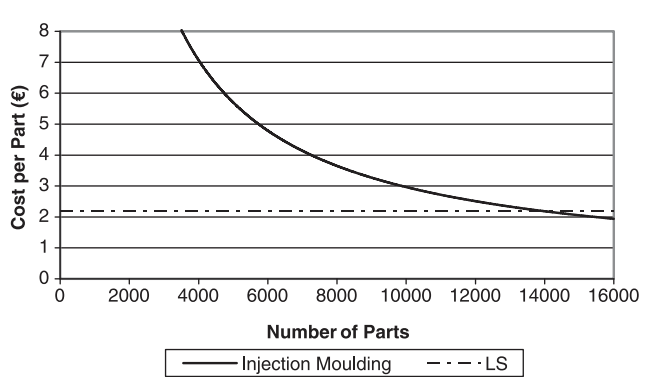
\includegraphics[width=0.6\textwidth]{./Images/HD.png}
\caption{Example of break-even analysis comparing LS with
IM}
\label{HD}
\caption*{\textbf{Source:} Cost estimation for rapid manufacturing ’ simultaneous production of mixed components using laser sintering \cite{ruffo2007cost}}
\end{figure}
\\
This model is a good approximation, but only validated when:
\begin{itemize}
    \item high production volumes
    \item production of the same piece
\end{itemize}

Later, in 2006, Ruffos \cite{ruffo2006cost}, a study based on the total cost, dividing them into labor, material, energy, administration and general costs.\cite{thomas2014costs,ruffo2007cost}\par
In contrast to the previous cost, developed by Hopkinson and Dickens, Ruffos' cost model has a curve that relates the cost per part to the volume of production and has the shape of a sawtooth. \cite{ruffo2007cost}\ref{Ruffos} \par
The Hopkinson and Dickens model was compared with that of Ruffos, now a comparison of evidence is an underestimation of the Hopkinson and Dickens model.\cite{thomas2014costs,ruffo2007cost}\par

\begin{figure}[h]
\centering
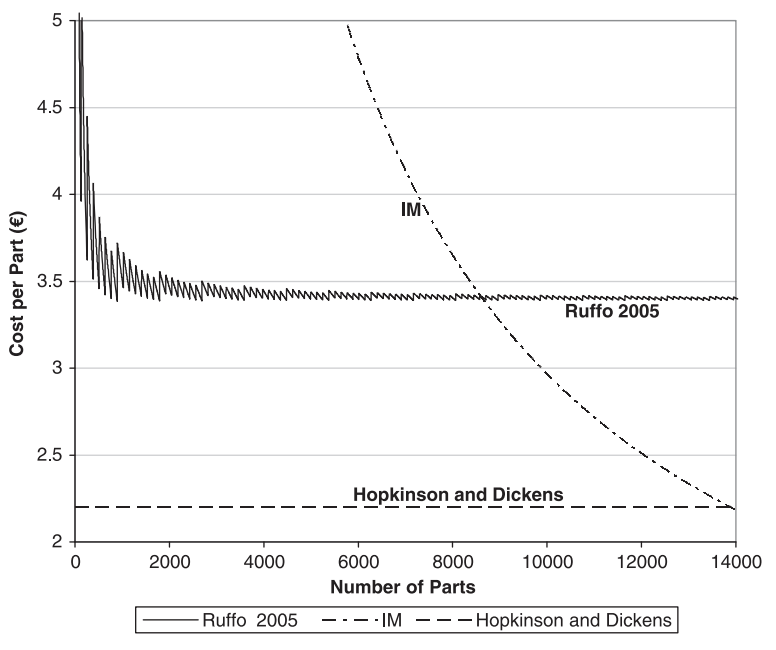
\includegraphics[width=0.5\textwidth]{./Images/3models.png}
\caption{Cost model comparison of \ac{LS} and \ac{IM}}
\label{Ruffos}
\caption*{\textbf{Source:} Cost estimation for rapid manufacturing ’ simultaneous production of mixed components using laser sintering \cite{ruffo2007cost}}
\end{figure}

Hopkinson, Dickens and Ruffos were the first to develop cost estimates for additive manufacturing. However, both authors developed models where they did not take into account the post processing of the parts, only the manufacture of the part.\par
Over the past decade, more complete new models have been developed. We can find quite complete models for certain production steps or for a specific production line.\par

Each piece has a set of production steps depending on its purpose and on the method used for its construction. A part produced with forging does not have the same post-processing as a part produced by \ac{AM}. Like a structural part, it does not have the same post-processing as a prototype. In this way, a flexible model is required where the editing of the production line of that particular part is allowed.\par
Therefore, the development of a cost model where the stages of manufacture can be selected is an important goal that has not been achieved and this is a gap extremelly important to fill in.

 % file "Thesis_Background.tex"
\cleardoublepage

%%%%%%%%%%%%%%%%%%%%%%%%%%%%%%%%%%%%%%%%%%%%%%%%%%%%%%%%%%%%%%%%%%%%%%%%
%                                                                      %
%     File: Thesis_Implementation.tex                                  %
%     Tex Master: Thesis.tex                                           %
%                                                                      %
%     Author: Andre C. Marta                                           %
%     Last modified :  2 Jul 2015                                      %
%                                                                      %
%%%%%%%%%%%%%%%%%%%%%%%%%%%%%%%%%%%%%%%%%%%%%%%%%%%%%%%%%%%%%%%%%%%%%%%%

\chapter{Implementation}
\label{chapter:implementation}

Insert your chapter material here...

%%%%%%%%%%%%%%%%%%%%%%%%%%%%%%%%%%%%%%%%%%%%%%%%%%%%%%%%%%%%%%%%%%%%%%%%
\section{Numerical Model}
\label{section:model}

Description of the numerical implementation of the models explained in Chapter~\ref{chapter:background}...


%%%%%%%%%%%%%%%%%%%%%%%%%%%%%%%%%%%%%%%%%%%%%%%%%%%%%%%%%%%%%%%%%%%%%%%%
\section{Verification and Validation}
\label{section:verification}

Basic test cases to compare the implemented model against other numerical tools (verification) and experimental data (validation)...

 % file "Thesis_Implementation.tex"
\cleardoublepage

%\input{Thesis_new_file} % add new .tex files for new chapters
% \cleardoublepage

%\input{Thesis_new_file} % add new .tex files for new chapters
% \cleardoublepage

%\input{Thesis_new_file} % add new .tex files for new chapters
% \cleardoublepage

%%%%%%%%%%%%%%%%%%%%%%%%%%%%%%%%%%%%%%%%%%%%%%%%%%%%%%%%%%%%%%%%%%%%%%%%
%                                                                      %
%     File: Thesis_Results.tex                                         %
%     Tex Master: Thesis.tex                                           %
%                                                                      %
%     Author: Andre C. Marta                                           %
%     Last modified :  2 Jul 2015                                      %
%                                                                      %
%%%%%%%%%%%%%%%%%%%%%%%%%%%%%%%%%%%%%%%%%%%%%%%%%%%%%%%%%%%%%%%%%%%%%%%%

\chapter{Results}
\label{chapter:results}

Insert your chapter material here...


%%%%%%%%%%%%%%%%%%%%%%%%%%%%%%%%%%%%%%%%%%%%%%%%%%%%%%%%%%%%%%%%%%%%%%%%
\section{Problem Description}
\label{section:problem}

Description of the baseline problem...


%%%%%%%%%%%%%%%%%%%%%%%%%%%%%%%%%%%%%%%%%%%%%%%%%%%%%%%%%%%%%%%%%%%%%%%%
\section{Baseline Solution}
\label{section:baseline}

Analysis of the baseline solution...


%%%%%%%%%%%%%%%%%%%%%%%%%%%%%%%%%%%%%%%%%%%%%%%%%%%%%%%%%%%%%%%%%%%%%%%%
\section{Enhanced Solution}
\label{section:enhanced}

Quest for the optimal solution...


% ----------------------------------------------------------------------
\subsection{Figures}
\label{subsection:figures}

Insert your section material and possibly a few figures...

Make sure all figures presented are referenced in the text!


% ----------------------------------------------------------------------
\subsubsection{Images}
\label{subsection:images}

\begin{figure}[!htb]
  \centering
  \includegraphics[width=0.25\textwidth]{Figures/Airbus_A350.jpg}
  \caption[Caption for figure in TOC.]{Caption for figure.}
  \label{fig:airbus1}
\end{figure}

\begin{figure}[!htb]
  \begin{subfigmatrix}{2}
    \subfigure[Airbus A320]{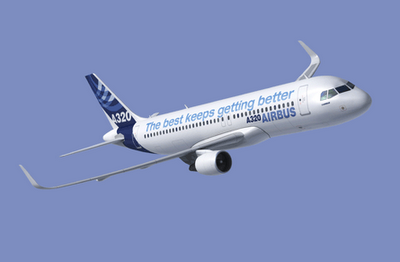
\includegraphics[width=0.49\linewidth]{Figures/Airbus_A320_sharklets.png}}
    \subfigure[Bombardier CRJ200]{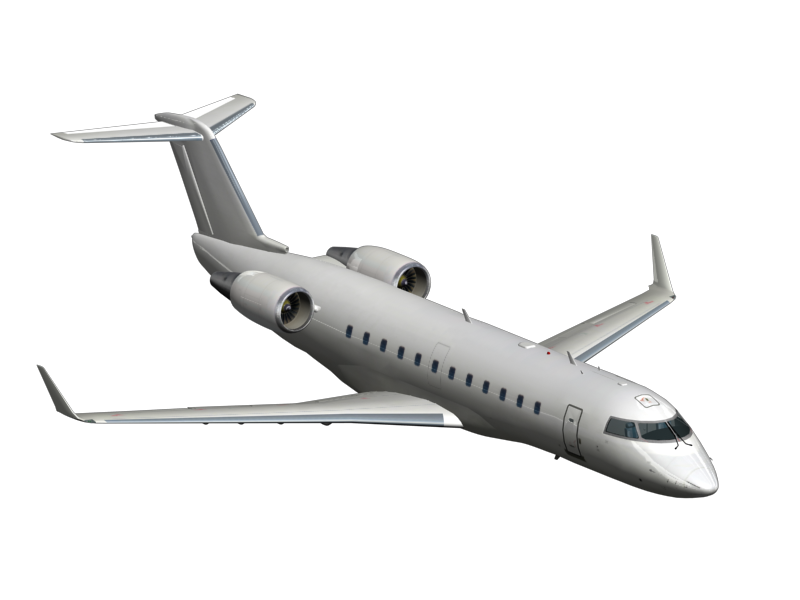
\includegraphics[width=0.49\linewidth]{Figures/Bombardier_CRJ200.png}}
  \end{subfigmatrix}
  \caption{Some aircrafts.}
  \label{fig:aircrafts}
\end{figure}

Make reference to Figures \ref{fig:airbus1} and \ref{fig:aircrafts}.

By default, the supported file types are {\it .png,.pdf,.jpg,.mps,.jpeg,.PNG,.PDF,.JPG,.JPEG}.

See \url{http://mactex-wiki.tug.org/wiki/index.php/Graphics_inclusion} for adding support to other extensions.


% ----------------------------------------------------------------------
\subsubsection{Drawings}
\label{subsection:drawings}

Insert your subsection material and for instance a few drawings...

The schematic illustrated in Fig.~\ref{fig:algorithm} can represent some sort of algorithm.

\begin{figure}[!htb]
  \centering
  \scriptsize
%  \footnotesize 
%  \small
  \setlength{\unitlength}{0.9cm}
  \begin{picture}(8.5,6)
    \linethickness{0.3mm}

    \put(3,6){\vector(0,-1){1}}
    \put(3.5,5.4){$\bf \alpha$}
    \put(3,4.5){\oval(6,1){}}
    %\put(0,4){\framebox(6,1){}}
    \put(0.3,4.4){Grid Generation: \quad ${\bf x} = {\bf x}\left({\bf \alpha}\right)$}

    \put(3,4){\vector(0,-1){1}}
    \put(3.5,3.4){$\bf x$}
    \put(3,2.5){\oval(6,1){}}
    %\put(0,2){\framebox(6,1){}}
    \put(0.3,2.4){Flow Solver: \quad ${\cal R}\left({\bf x},{\bf q}\left({\bf x}\right)\right) = 0$}

    \put(6.0,2.5){\vector(1,0){1}}
    \put(6.4,3){$Y_1$}

    \put(3,2){\vector(0,-1){1}}
    \put(3.5,1.4){$\bf q$}
    \put(3,0.5){\oval(6,1){}}
    %\put(0,0){\framebox(6,1){}}
    \put(0.3,0.4){Structural Solver: \quad ${\cal M}\left({\bf x},{\bf q}\left({\bf x}\right)\right) = 0$}

    \put(6.0,0.5){\vector(1,0){1}}
    \put(6.4,1){$Y_2$}

    %\put(7.8,2.5){\oval(1.6,5){}}
    \put(7.0,0){\framebox(1.6,5){}}
    \put(7.1,2.5){Optimizer}
    \put(7.8,5){\line(0,1){1}}
    \put(7.8,6){\line(-1,0){4.8}}
  \end{picture}
  \caption{Schematic of some algorithm.}
  \label{fig:algorithm}
\end{figure}


% ----------------------------------------------------------------------
\subsection{Equations}
\label{subsection:equations}

Equations can be inserted in different ways.

The simplest way is in a separate line like this

\begin{equation}
  \frac{{\rm d} q_{ijk}}{{\rm d} t} + {\cal R}_{ijk}({\bf q}) = 0 \,.
\label{eq:ode}
\end{equation}

If the equation is to be embedded in the text. One can do it like this ${\partial {\cal R}}/{\partial {\bf q}}=0$.

It may also be split in different lines like this

\begin{eqnarray}
  {\rm Minimize}   && Y({\bf \alpha},{\bf q}({\bf \alpha}))            \nonumber           \\
  {\rm w.r.t.}     && {\bf \alpha} \,,                                 \label{eq:minimize} \\
  {\rm subject~to} && {\cal R}({\bf \alpha},{\bf q}({\bf \alpha})) = 0 \nonumber           \\
                   &&       C ({\bf \alpha},{\bf q}({\bf \alpha})) = 0 \,. \nonumber
\end{eqnarray}

It is also possible to use subequations. Equations~\ref{eq:continuity}, \ref{eq:momentum} and \ref{eq:energy} form the Naver--Stokes equations~\ref{eq:NavierStokes}.

\begin{subequations}
    \begin{equation}
    \frac{\partial \rho}{\partial t} + \frac{\partial}{\partial x_j}\left( \rho u_j \right) = 0 \,,
    \label{eq:continuity}
    \end{equation}
    \begin{equation}
    \frac{\partial}{\partial t}\left( \rho u_i \right) + \frac{\partial}{\partial x_j} \left( \rho u_i u_j + p \delta_{ij} - \tau_{ji} \right) = 0, \quad i=1,2,3 \,,
    \label{eq:momentum}
    \end{equation}
    \begin{equation}
        \frac{\partial}{\partial t}\left( \rho E \right) + \frac{\partial}{\partial x_j} \left( \rho E u_j + p u_j - u_i \tau_{ij} + q_j \right) = 0 \,.
    \label{eq:energy}
    \end{equation}
\label{eq:NavierStokes}%
\end{subequations}


% ----------------------------------------------------------------------
\subsection{Tables}
\label{section:tables}

Insert your subsection material and for instance a few tables...

Make sure all tables presented are referenced in the text!

Follow some guidelines when making tables:

\begin{itemize}
  \item Avoid vertical lines
  \item Avoid “boxing up” cells, usually 3 horizontal lines are enough: above, below, and after heading
  \item Avoid double horizontal lines
  \item Add enough space between rows
\end{itemize}

\begin{table}[!htb]
  \renewcommand{\arraystretch}{1.2} % more space between rows
  \centering
  \begin{tabular}{lccc}
    \toprule
    Model           & $C_L$ & $C_D$ & $C_{M y}$ \\
    \midrule
    Euler           & 0.083 & 0.021 & -0.110    \\
    Navier--Stokes  & 0.078 & 0.023 & -0.101    \\
    \bottomrule
  \end{tabular}
  \caption[Table caption shown in TOC.]{Table caption.}
  \label{tab:aeroCoeff}
\end{table}

Make reference to Table \ref{tab:aeroCoeff}.

Tables \ref{tab:memory} and \ref{tab:multipleColumns} are examples of tables with merging columns:

\begin{table}[!htb]
  \renewcommand{\arraystretch}{1.2} % more space between rows
  \centering
  \begin{tabular}[]{lrr}
    \toprule
                & \multicolumn{2}{c}{\underline{Virtual memory [MB]}} \\
                & Euler       & Navier--Stokes \\
    \midrule
      Wing only &  1,000      &    2,000       \\
      Aircraft  &  5,000      &   10,000       \\
      (ratio)   & $5.0\times$ & $5.0\times$    \\
    \bottomrule
  \end{tabular}
  \caption{Memory usage comparison (in MB).}
  \label{tab:memory}
\end{table}

\begin{table}[!htb]
  \centering
  \renewcommand{\arraystretch}{1.2} % more space between rows
  \begin{tabular}{@{}rrrrcrrr@{}} % remove space to the vertical edges @{}...@{}
    \toprule
      & \multicolumn{3}{c}{$w = 2$} & \phantom{abc} & \multicolumn{3}{c}{$w = 4$} \\
    \cmidrule{2-4}
    \cmidrule{6-8}
      & $t=0$ & $t=1$ & $t=2$ && $t=0$ & $t=1$ & $t=2$ \\
    \midrule
      $dir=1$
      \\
      $c$ &  0.07 &  0.16 &  0.29 &&  0.36 &  0.71 &   3.18 \\
      $c$ & -0.86 & 50.04 &  5.93 && -9.07 & 29.09 &  46.21 \\
      $c$ & 14.27 &-50.96 &-14.27 && 12.22 &-63.54 &-381.09 \\
      $dir=0$
      \\
      $c$ &  0.03 &  1.24 &  0.21 &&  0.35 & -0.27 &  2.14 \\
      $c$ &-17.90 &-37.11 &  8.85 &&-30.73 & -9.59 & -3.00 \\
      $c$ &105.55 & 23.11 &-94.73 &&100.24 & 41.27 &-25.73 \\
    \bottomrule
  \end{tabular}
  \caption{Another table caption.}
  \label{tab:multipleColumns}
\end{table}

An example with merging rows can be seen in Tab.\ref{tab:multipleRows}.

\begin{table}[!htb]
  \renewcommand{\arraystretch}{1.2} % more space between rows
  \centering
  \begin{tabular}{ccccc}
    \toprule
      \multirow{2}{*}{ABC} & \multicolumn{4}{c}{header} \\
      \cmidrule{2-5} & 1.1 & 2.2 & 3.3 & 4.4 \\
    \midrule
      \multirow{2}{*}{IJK} & \multicolumn{2}{c}{\multirow{2}{*}{group}} & 0.5 & 0.6 \\
      \cmidrule{4-5}       & \multicolumn{2}{c}{}                       & 0.7 & 1.2 \\
    \bottomrule
  \end{tabular}
  \caption{Yet another table caption.}
  \label{tab:multipleRows}
\end{table}

If the table has too many columns, it can be scaled to fit the text widht, as in Tab.\ref{tab:scale}.
\begin{table}[!htb]
  \renewcommand{\arraystretch}{1.2} % more space between rows
  \centering
  \resizebox*{\textwidth}{!}{%
    \begin{tabular}[]{lcccccccccc}
      \toprule
        Variable &  a  &  b  &  c  &  d  &  e  &  f  &  g  &  h  &  i  &  j  \\
      \midrule
        Test 1   &  10,000 &  20,000 &  30,000 &  40,000 &  50,000 &  60,000 &  70,000 &  80,000 &  90,000 & 100,000 \\
        Test 2   &  20,000 &  40,000 &  60,000 &  80,000 & 100,000 & 120,000 & 140,000 & 160,000 & 180,000 & 200,000 \\
      \bottomrule
    \end{tabular}
  }%
  \caption{Very wide table.}
  \label{tab:scale}%
\end{table}


% ----------------------------------------------------------------------
\subsection{Mixing}
\label{section:mixing}

If necessary, a figure and a table can be put side-by-side as in Fig.\ref{fig:side_by_side}

\begin{figure}[!htb]
  \begin{minipage}[b]{0.60\linewidth}
    \centering
    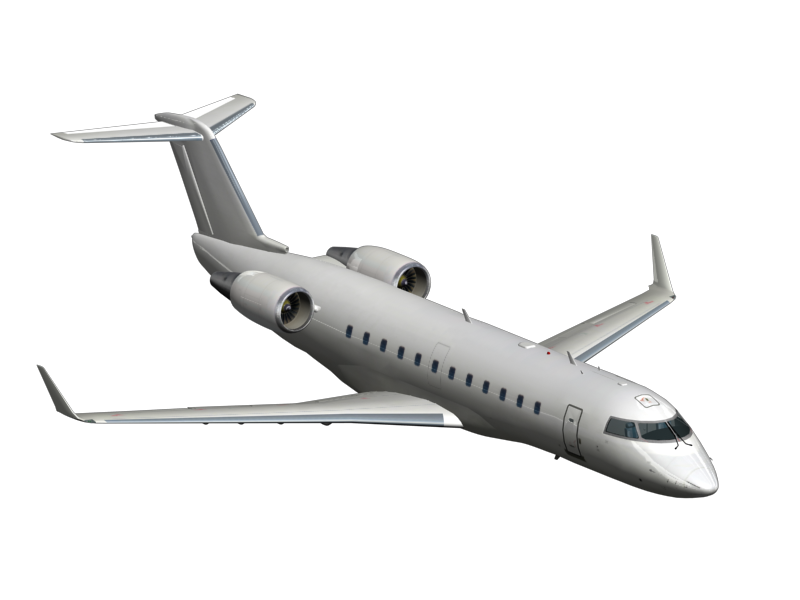
\includegraphics[width=\linewidth]{Figures/Bombardier_CRJ200}
  \end{minipage}%
  \begin{minipage}[b]{0.30\linewidth}
    \centering
    \begin{tabular}[b]{lll}
      \toprule
        \multicolumn{3}{c}{Legend} \\
      \midrule
        A & B & C \\
        0 & 0 & 0 \\
        0 & 1 & 0 \\
        1 & 0 & 0 \\
        1 & 1 & 1 \\
      \bottomrule
    \end{tabular}
    \vspace{5em}
  \end{minipage}
\caption{Figure and table side-by-side.}
\label{fig:side_by_side}
\end{figure}

 % file "Thesis_Results.tex"
\cleardoublepage

%%%%%%%%%%%%%%%%%%%%%%%%%%%%%%%%%%%%%%%%%%%%%%%%%%%%%%%%%%%%%%%%%%%%%%%%
%                                                                      %
%     File: Thesis_Conclusions.tex                                     %
%     Tex Master: Thesis.tex                                           %
%                                                                      %
%     Author: Andre C. Marta                                           %
%     Last modified :  2 Jul 2015                                      %
%                                                                      %
%%%%%%%%%%%%%%%%%%%%%%%%%%%%%%%%%%%%%%%%%%%%%%%%%%%%%%%%%%%%%%%%%%%%%%%%

\chapter{Conclusions}
\label{chapter:conclusions}

Insert your chapter material here...


% ----------------------------------------------------------------------
\section{Achievements}
\label{section:achievements}

The major achievements of the present work...


% ----------------------------------------------------------------------
\section{Future Work}
\label{section:future}

A few ideas for future work...

 % file "Thesis_Conclusions.tex"
\cleardoublepage

% ----------------------------------------------------------------------
%  Bibliography
% ----------------------------------------------------------------------

% Add entry in the table of contents as chapter
\phantomsection
\addcontentsline{toc}{chapter}{\bibname}

% Include all references in .bib file, even non-cited ones...
%\nocite{*} % this should be used carefully because it is not correct!

% Produces the bibliography section when processed by BibTeX
%
% Bibliography style
% > entries ordered alphabetically
%\bibliographystyle{plain}
% > unsorted with entries appearing in the order in which the citations appear.
%\bibliographystyle{unsrt}
% > entries ordered alphabetically, with first names and names of journals and months abbreviated
%\bibliographystyle{abbrv}
% > entries ordered alphabetically, with reference markers based on authors' initials and publication year
%\bibliographystyle{alpha}
%
% Replacement bibliography styles provided by 'natbib' package
% (plainnat.bst, abbrvnat.bst, unsrtnat.bst )
% > entries ordered alphabetically
%\bibliographystyle{plainnat}
% > unsorted with entries appearing in the order in which the citations appear.
%\bibliographystyle{unsrtnat}
% > entries ordered alphabetically, with first names and names of journals and months abbreviated
%\bibliographystyle{abbrvnat} % <<<<< SELECT IF USING REFERENCES BY AUTHOR/YEAR
% > entries ordered alphabetically, with reference markers based on authors' initials and publication year
%\bibliographystyle{alpha}
%
% Custom bibliography style adapted from 'natbib' package
%   (based on http://tex.stackexchange.com/questions/5053/is-it-possible-to-get-unsrt-abbrv-bibliography)
%   (unsrtnat.bst + abbrvnat.bst -> abbrvunsrtnat.bst)
%   (original files copied from:
%   http://tug.ctan.org/macros/latex/contrib/natbib/abbrvnat.bst
%   http://tug.ctan.org/macros/latex/contrib/natbib/unsrtnat.bst
% > unsorted with entries appearing in the order in which the citations appear, with first names and names of journals and months abbreviated.
\bibliographystyle{abbrvunsrtnat} % <<<<< SELECT IF USING REFERENCES BY NUMBER (CITATION ORDER)

% External bibliography database file in the BibTeX format
\bibliography{Thesis_bib_DB} % file "Thesis_bib_DB.bib"

\cleardoublepage

% ----------------------------------------------------------------------
%  Appendix (optional)
%
%  CAUTION: 1) the main document (up to the conclusions) shall not exceed 80 pages
%           2) the document shall not exceed a total of 100 pages (per IST regulations)
% ----------------------------------------------------------------------
\appendix

% add page number prefix according to apendix chapter (optional)
%\renewcommand{\thepage}{\thechapter.\arabic{page}}

% re-set arabic numbering (A.1,A.2,...) (optional, use only if chapter prefix is added)
%\setcounter{page}{1}

%%%%%%%%%%%%%%%%%%%%%%%%%%%%%%%%%%%%%%%%%%%%%%%%%%%%%%%%%%%%%%%%%%%%%%%%
%                                                                      %
%     File: Thesis_Appendix_A.tex                                      %
%     Tex Master: Thesis.tex                                           %
%                                                                      %
%     Author: Andre C. Marta                                           %
%     Last modified :  2 Jul 2015                                      %
%                                                                      %
%%%%%%%%%%%%%%%%%%%%%%%%%%%%%%%%%%%%%%%%%%%%%%%%%%%%%%%%%%%%%%%%%%%%%%%%

\chapter{Vector calculus}
\label{chapter:appendixVectors}

In case an appendix if deemed necessary, the document cannot exceed a total of 100 pages...

Some definitions and vector identities are listed in the section below.

% ----------------------------------------------------------------------
\section{Vector identities}
\label{section:vectorIdentities}

\begin{equation}
	\nabla \times \left( \nabla \phi \right) = 0
	\label{eq:cross_nnp}
\end{equation}

\begin{equation}
	\nabla \cdot \left( \nabla \times {\bf u} \right) = 0
	\label{eq:dotCross_nnu}
\end{equation}

 % file "Thesis_Appendix_A.tex"
\cleardoublepage

% re-set arabic numbering (B.1,B.2,...) (optional, use only if chapter prefix is added)
%\setcounter{page}{1}

%%%%%%%%%%%%%%%%%%%%%%%%%%%%%%%%%%%%%%%%%%%%%%%%%%%%%%%%%%%%%%%%%%%%%%%%
%                                                                      %
%     File: Thesis_Appendix_B.tex                                      %
%     Tex Master: Thesis.tex                                           %
%                                                                      %
%     Author: Andre C. Marta                                           %
%     Last modified :  2 Jul 2015                                      %
%                                                                      %
%%%%%%%%%%%%%%%%%%%%%%%%%%%%%%%%%%%%%%%%%%%%%%%%%%%%%%%%%%%%%%%%%%%%%%%%

\chapter{Technical Datasheets}
\label{chapter:appendixDatasheets}

It is possible to add PDF files to the document, such as technical sheets of some equipment used in the work.

% ----------------------------------------------------------------------
\section{Some Datasheet}
\label{section:datasheet}

% See more options to include PDF files in
% http://mirror.unl.edu/ctan/macros/latex/contrib/pdfpages/pdfpages.pdf
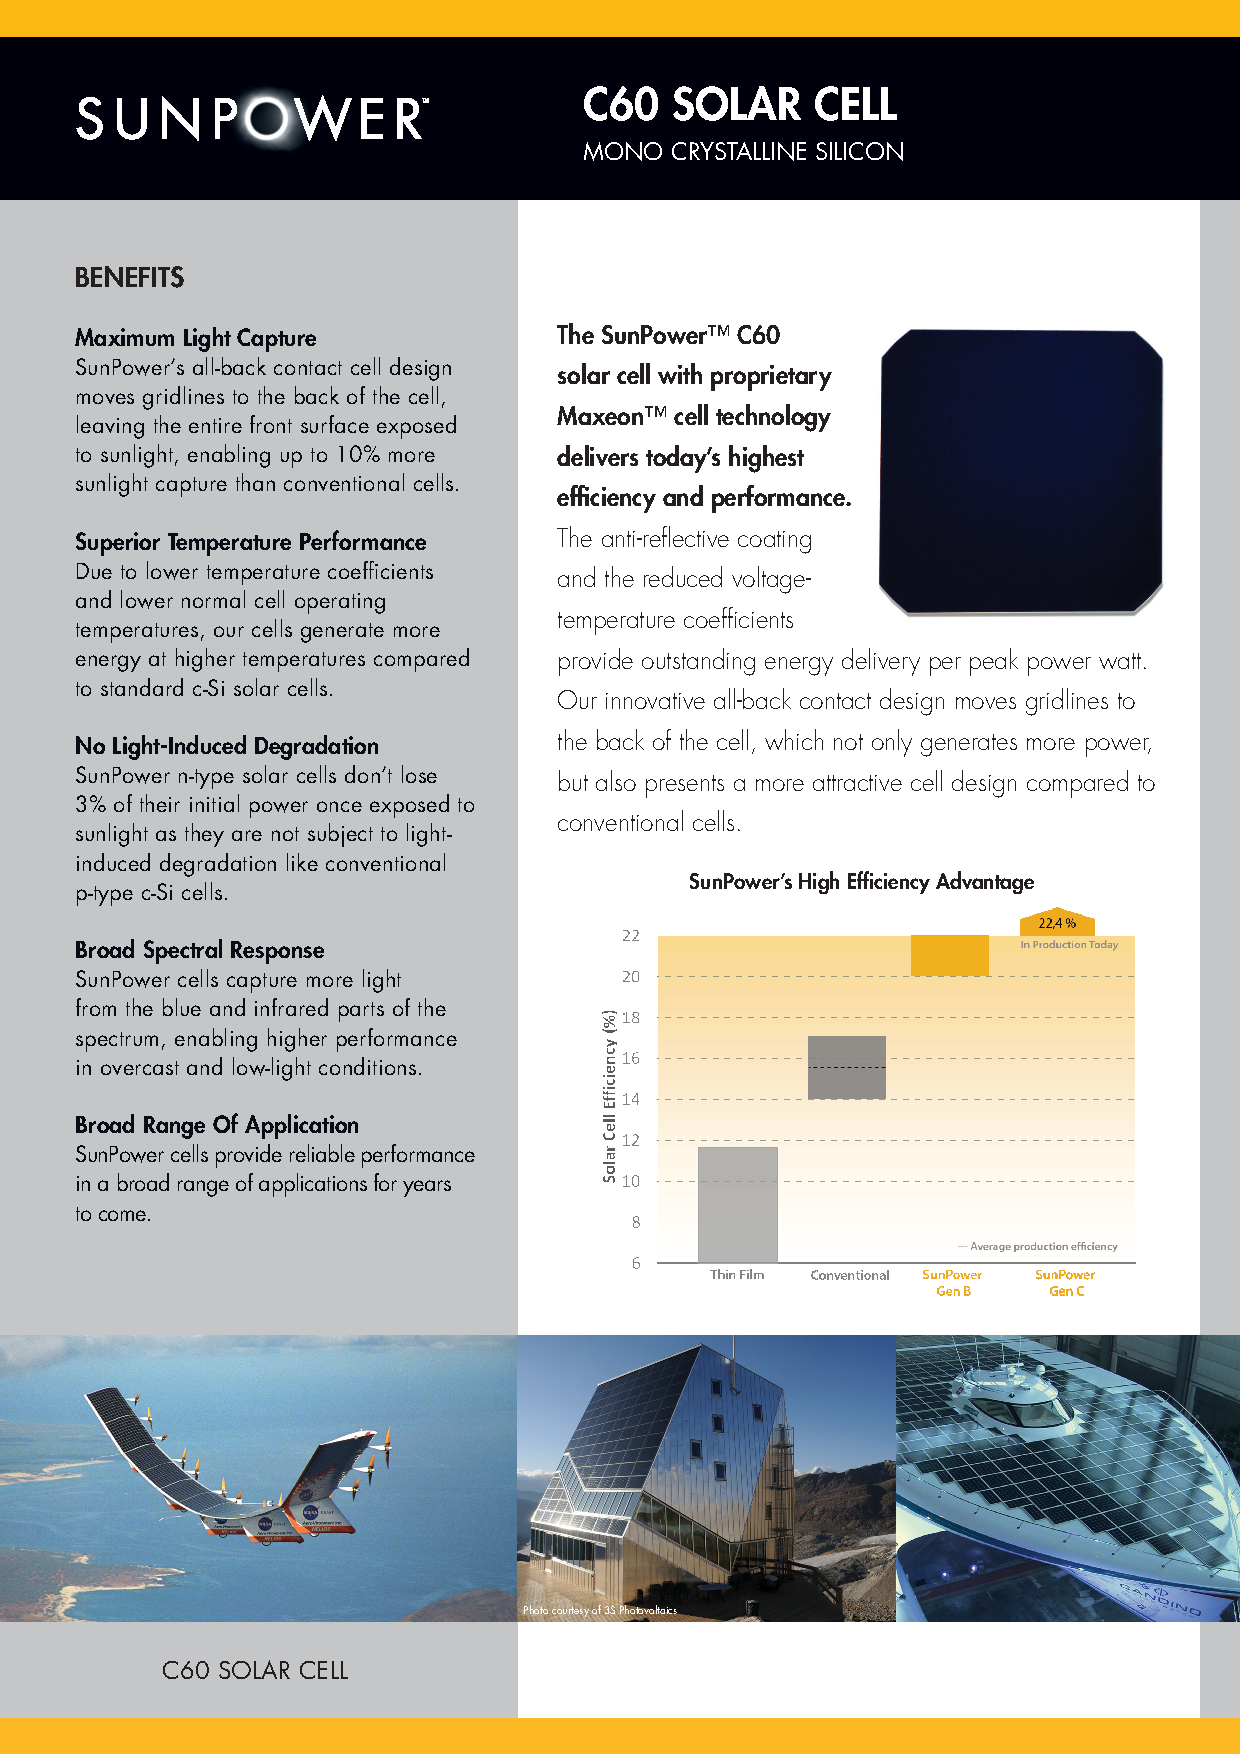
\includepdf[pages={1-2},nup=1x2,landscape=true]{Figures/SolarCell_Sunpower_C60.pdf}

 % file "Thesis_Appendix_B.tex"
\cleardoublepage

% ----------------------------------------------------------------------
\end{document}
% ----------------------------------------------------------------------

